\documentclass[nopacs,amsmath,amsfonts,amssymb,aps,superscriptaddress]{revtex4}
%%% use showpacs if we want to display it

\setlength{\paperheight}{11in}
\usepackage{amsthm}
\newtheorem{proposition}{Proposition}[section]
\usepackage{tabularx}
\usepackage[dvipsnames]{xcolor}

\usepackage{todonotes}
\usepackage{upgreek}
\usepackage{graphicx}% Include figure files
\graphicspath{{figs/}}% figures live in the figs/ subdirectory
\usepackage{float}
\usepackage{tikz}
\newtheorem{corollary}{Corollary}[section]
\begin{document}

\title{Spectral Green functions for T-duality-regularised electrostatics in finite and bounded planar geometries}

\author{Davide Batic}
\email{davide.batic@ku.ac.ae}
\affiliation{Mathematics Department, Khalifa University of Science and Technology, PO Box 127788, Abu Dhabi, United Arab Emirates}

\author{Denys Dutykh}
\email{denys.dutykh@ku.ac.ae}
\affiliation{Mathematics Department, Khalifa University of Science and Technology, PO Box 127788, Abu Dhabi, United Arab Emirates}
\date{\today}

\begin{abstract}
We develop a finite-size formulation of T-duality-deformed electrostatics in $(2+1)$ dimensions. The T-duality form factor regularises the ultraviolet behaviour of the planar static Green function, while finite volume and boundary conditions control the infrared sector. We first rederive the self-energy-subtracted infinite-plane interaction, which is finite at the origin and recovers the logarithmic Coulomb law at large distances. We then define the corresponding Green function on general domains via the spectral calculus of the Laplacian and work out explicit realisations on the square torus, the grounded half-plane, and the grounded strip. The torus implements charge neutrality through zero-mode subtraction, whereas Dirichlet boundaries produce finite image and self-energy effects. Finally, we introduce an additive-constant-free running interaction dimension and show that the ultraviolet flow to one dimension survives in finite volume, while the infrared behaviour is geometry-dependent.
\end{abstract}

\maketitle

\section{Introduction}

In two spatial dimensions, electrostatics occupies a marginal position: the Green function of the Laplacian is neither Coulombic nor linearly confining, but logarithmic. This elementary fact makes $(2+1)$-dimensional electrodynamics an unusually sensitive arena for testing ultraviolet regularisation, infrared boundary conditions, and the interplay between local gauge dynamics and nonlocal modifications. It also gives the theory a double physical relevance. On the high energy side, three-dimensional gauge theories exhibit distinctive infrared and topological features, including gauge invariant mass generation through Chern–Simons terms and nontrivial compact-gauge-field effects \cite{DeserJackiwTempleton1982, Polyakov1975}. On the condensed matter side, planar electromagnetic kernels appear in thin films, vortices, quantum Hall systems, strange metals, and other effectively two-dimensional media, where sample geometry and boundary conditions are not idealisations but part of the physical problem \cite{Pearl1964, KosterlitzThouless1973, LaNaveLimtragoolPhillips2019}. A further motivation comes from the use of nonlocal kernels as effective descriptions of short-distance physics. In string theory, T-duality relates compactification radii $R$ and $\alpha'/R$, thereby tying ultraviolet and infrared scales in a way that has no point particle analogue \cite{Sathiapalan1987, GiveonPorratiRabinovici1994}. Padmanabhan’s path integral duality proposal implements a closely related idea at the level of particle propagation, namely, that invariance under an inversion of path length introduces a zero-point length and modifies the propagator with a Bessel function form factor \cite{Padmanabhan1997}. Subsequent work connected this zero-point length structure to string fluctuations and T-duality corrections \cite{SmailagicSpallucciPadmanabhan2003, FontaniniSpallucciPadmanabhan2006}. In field theoretic applications, the same mechanism has been used to regularise static gravitational and electromagnetic potentials, replacing point source singularities by finite short-distance profiles controlled by a length $\ell_0$ \cite{NicoliniSpallucciWondrak2019, GaeteNicolini2022}. The planar case is especially delicate. In ordinary $(2+1)$-dimensional Maxwell theory, the static potential between charges behaves as $\ln{(\mu r)}$, where $\mu$ is an infrared scale. Thus, the same logarithm encodes both short-distance and long-distance singular behaviour. Recent work on T-duality-deformed $(2+1)$-dimensional electrodynamics showed that the zero-point length kernel softens the short-distance behaviour while retaining the logarithmic large distance growth \cite{GaeteNicolini2026}. However, the infinite plane is not the natural endpoint of the problem. The persistence of the infrared logarithm means that any physical prediction requires either an infrared prescription, a neutralising background, or a finite geometry. This issue is not merely technical because, in finite planar samples, the allowed modes, zero-mode subtraction, and boundary conditions determine the electrostatic energy.

The present work addresses this gap by formulating T-duality-deformed planar electrostatics directly on finite and bounded domains. Rather than imposing the T-duality form factor only in momentum space on $\mathbb{R}^2$, we define the nonlocal static kernel through the spectral calculus of the Laplacian on a domain $\Omega$. If $-\nabla_\Omega^2 u_n=\lambda_n u_n$, the T-duality Green function is obtained by weighting each nonzero mode with the factor $\ell_0\sqrt{\lambda_n}K_1(\ell_0\sqrt{\lambda_n})/\lambda_n$. This construction is natural for self-adjoint elliptic operators and parallels standard treatments of fractional and nonlocal operators on bounded domains \cite{CaffarelliSilvestre2007, BonitoPasciak2015}. It also makes explicit which part of the physics is universal (the ultraviolet smoothing controlled by $\ell_0$) and which part is geometry-dependent (the infrared spectrum and the boundary response). Our central question is therefore how the T-duality length $\ell_0$ modifies electrostatic interactions in finite $(2+1)$-dimensional geometries, and how the familiar logarithmic potential and its regularised short-distance limit are recovered when the system size is taken to infinity? We answer this by deriving the spectral Green function for general domains, then working out explicit finite-volume and boundary examples. The square torus provides a controlled infrared regulator via zero-mode removal and yields an exact mode-sum expression for the self-energy-subtracted pair potential. The grounded half-plane and related geometries isolate boundary effects and clarify when image-type constructions survive the nonlocal deformation. This is important because nonlocal electrodynamics need not obey the same boundary intuitions as local Maxwell theory. Notice that in related nonlocal models, the usual image method can fail \cite{BorgesBufalo2025}. The purpose of this paper is to provide a reproducible finite-size framework for T-duality-deformed $(2+1)$-dimensional electrodynamics. The construction gives well-defined interaction energies in finite samples, identifies the infinite-plane potential as a controlled limit, and separates ultraviolet regularisation from infrared geometry. Beyond its role as a consistency check on the planar T-duality kernel, the analysis is intended to make the model usable in contexts where boundaries, sample size, and mode discreteness are experimentally meaningful, particularly in effective planar condensed matter systems.

The paper is organised as follows. We first review the static T-duality kernel and its corrected infinite-plane Green function. We then define the spectral Green function on a general domain, derive the toroidal finite-volume potential, and analyse boundary geometries such as the half-plane. We close by discussing finite-size corrections, dimensional-flow diagnostics, and possible condensed-matter applications.

\section{T-duality kernel and corrected infinite-plane Green function}

The starting point is the T-duality-modified Abelian gauge theory obtained by replacing the Maxwell kinetic operator by a nonlocal form factor. In the static sector, the relevant operator is a function of the positive spatial Laplacian, and we write
\begin{equation}
  f_{\ell_0}(k)\equiv f(k):=\ell_0 k K_1(\ell_0 k),
  \qquad k=|\mathbf k|,
\end{equation}
with the continuous extension $f_{\ell_0}(0)=1$. Here $K_1$ is the modified Bessel function of the second kind and $\ell_0$ is the zero-point length. The same form factor appears in Padmanabhan's path-integral-duality propagator and in its string-theoretic T-duality realisation \cite{Padmanabhan1997, SmailagicSpallucciPadmanabhan2003, FontaniniSpallucciPadmanabhan2006}. In the gauge theory implementation, the free Lagrangian may be written schematically as
\begin{equation}
  \mathcal L_{\rm free}=-\frac{1}{4} F_{\mu\nu}\mathcal O F^{\mu\nu},\qquad
  \mathcal O=\left[\ell_0\sqrt{\Delta} K_1\left(\ell_0\sqrt{\Delta}\right)\right]^{-1},
\end{equation}
with $\Delta$ replaced by $-\nabla^2$ for static Euclidean spatial configurations. This construction was used previously to regularise four-dimensional electrostatic and gravitational potentials \cite{NicoliniSpallucciWondrak2019, GaeteNicolini2022}, and more recently to study the marginal $(2+1)$-dimensional case \cite{GaeteNicolini2026}. For conserved external sources, the longitudinal part of the gauge propagator does not contribute. The static interaction between two point charges therefore reduces to a scalar Green function with momentum-space kernel
\begin{equation}
  \widetilde G_{\infty,\ell_0}(\mathbf k)
  =\frac{f_{\ell_0}(k)}{k^2}
  =\frac{\ell_0 k K_1(\ell_0 k)}{k^2},
  \qquad k\neq 0.
\end{equation}
The exclusion of $k=0$ is the usual two-dimensional zero-mode ambiguity: in position space it is the freedom to add an arbitrary constant to the Green function, or equivalently to add $(2\pi)^2 C\delta^{(2)}(\mathbf k)$ in momentum space.

We use the Fourier convention
\begin{equation}
  \widehat u(\mathbf k)=\int_{\mathbb R^2}u(\mathbf x)e^{-i\mathbf k\cdot\mathbf x}\,d^2x,
  \qquad
  u(\mathbf x)=\int_{\mathbb R^2}\frac{d^2k}{(2\pi)^2}\widehat u(\mathbf k)e^{i\mathbf k\cdot\mathbf x}.
\end{equation}
Thus a formal zero-mode-regulated representative of the infinite-plane Green function is
\begin{equation}
  G_{\infty,\ell_0}(\mathbf r)
  =\int\frac{d^2 k}{(2\pi)^2}\frac{\ell_0 k K_1(\ell_0 k)}{k^2}e^{i\mathbf k\cdot \mathbf r}+C.
\end{equation}
For two static charges $Q$ and $Q'$, separated by $\mathbf r=\mathbf x_1-\mathbf x_2$, the cross-term interaction is
\begin{equation}
  V_{\rm int}(r)=Q Q' G_{\infty,\ell_0}(r).
\end{equation}
In two spatial dimensions $G_{\infty,\ell_0}(r)$ is not itself an infrared-finite quantity. Indeed, since $\ell_0 k K_1(\ell_0 k)\to 1$ as $k\to 0$, the integrand behaves as $1/k^2$ at small momentum, and the radial integral contains the usual logarithmic zero-mode divergence. The physically meaningful free-space quantity for a neutral pair is therefore the self-energy-subtracted difference
\begin{equation}
  G_{\infty,\ell_0}(r)-G_{\infty,\ell_0}(0)
  =\int\frac{d^2 k}{(2\pi)^2}\frac{\ell_0 k K_1(\ell_0 k)}{k^2}
  \left(e^{i\mathbf k\cdot\mathbf r}-1\right),
\end{equation}
which is finite for all $r$. Equivalently, for opposite charges $Q'=-Q$, we define the positive separation energy
\begin{equation}
  \Delta V_{\infty,\ell_0}(r)
  \equiv V_{\rm int}(r)-V_{\rm int}(0)
  =Q^2\left[G_{\infty,\ell_0}(0)-G_{\infty,\ell_0}(r)\right].
\end{equation}
The following proposition collects the exact source smearing, the zero-mode statement, and the resulting subtracted interaction.

\begin{proposition}\label{prop:infinite-plane-td}
Let $\ell_0>0$ and let $f_{\ell_0}(k)=\ell_0 kK_1(\ell_0 k)$, with $f_{\ell_0}(0)=1$ by continuous extension. Define the T-duality-smeared source
\begin{equation}
  \rho_{\ell_0}(\mathbf x)
  =\int_{\mathbb R^2}\frac{d^2k}{(2\pi)^2}f_{\ell_0}(k)e^{i\mathbf k\cdot\mathbf x}.
\end{equation}
Then, with $r=|\mathbf x|$,
\begin{equation}\label{density}
  \rho_{\ell_0}(r)
  =\frac{1}{\pi\ell_0^2}\left(1+\frac{r^2}{\ell_0^2}\right)^{-2},
  \qquad
  \int_{\mathbb R^2}\rho_{\ell_0}(\mathbf x)\,d^2x=1.
\end{equation}
Let $G_{\infty,\ell_0}$ be a radial distributional solution of
\begin{equation}\label{Poisson}
  -\nabla^2G_{\infty,\ell_0}(\mathbf r)=\rho_{\ell_0}(\mathbf r),
\end{equation}
whose Fourier transform satisfies
\begin{equation}
  \widehat G_{\infty,\ell_0}(\mathbf k)
  =\frac{f_{\ell_0}(k)}{k^2},
  \qquad k\neq 0,
\end{equation}
with the freedom to add a zero-mode term $(2\pi)^2C\delta^{(2)}(\mathbf k)$. Then $G_{\infty,\ell_0}$ is unique up to an additive constant, and
\begin{equation}\label{equa}
  \frac{dG_{\infty,\ell_0}}{dr}
  =-\frac{r}{2\pi(r^2+\ell_0^2)},
  \qquad
  G_{\infty,\ell_0}(0)-G_{\infty,\ell_0}(r)
  =\frac{1}{4\pi}\ln\left(1+\frac{r^2}{\ell_0^2}\right).
\end{equation}
For a neutral pair with charges $Q$ and $-Q$, the self-energy-subtracted separation energy is
\begin{equation}\label{DeltaV}
  \Delta V_{\infty,\ell_0}(r)
  =Q^2\left[G_{\infty,\ell_0}(0)-G_{\infty,\ell_0}(r)\right]
  =\frac{Q^2}{4\pi}\ln\left(1+\frac{r^2}{\ell_0^2}\right).
\end{equation}
Moreover,
\begin{equation}
  \Delta V_{\infty,\ell_0}(r)
  =\frac{Q^2}{4\pi}\left[
  \frac{r^2}{\ell_0^2}-\frac{r^4}{2\ell_0^4}
  +\mathcal O\left(\frac{r^6}{\ell_0^6}\right)\right],
  \qquad r\ll\ell_0,
\end{equation}
while
\begin{equation}
  \Delta V_{\infty,\ell_0}(r)
  =\frac{Q^2}{2\pi}\ln\left(\frac r{\ell_0}\right)
  +\frac{Q^2\ell_0^2}{4\pi r^2}
  +\mathcal O\left(\frac{\ell_0^4}{r^4}\right),
  \qquad r\gg\ell_0.
\end{equation}
\end{proposition}

\begin{proof}
We use the Schwinger--Basset representation
\begin{equation}
  zK_1(z)=\int_0^\infty d\alpha\,
  \exp\left(-\alpha-\frac{z^2}{4\alpha}\right),
  \qquad z>0,
\end{equation}
which is a special case of the integral representations of $K_\nu$ \cite{DLMF}. With $z=\ell_0 k$, this gives
\begin{equation}
  \rho_{\ell_0}(\mathbf r)
  =\int_0^\infty d\alpha\,e^{-\alpha}
  \int\frac{d^2k}{(2\pi)^2}
  \exp\left(-\frac{\ell_0^2k^2}{4\alpha}+i\mathbf k\cdot\mathbf r\right).
\end{equation}
The Gaussian integral is
\begin{equation}\label{GE}
  \int\frac{d^2 k}{(2\pi)^2}\exp\left(-a k^2+i\mathbf k\cdot\mathbf r\right)
  =\frac{1}{4\pi a}\exp\left(-\frac{r^2}{4a}\right),
  \qquad a=\frac{\ell_0^2}{4\alpha}.
\end{equation}
Therefore
\begin{equation}
  \rho_{\ell_0}(r)
  =\frac{1}{\pi\ell_0^2}\int_0^\infty d\alpha\,\alpha
  \exp\left[-\alpha\left(1+\frac{r^2}{\ell_0^2}\right)\right]
  =\frac{1}{\pi\ell_0^2}\left(1+\frac{r^2}{\ell_0^2}\right)^{-2}.
\end{equation}
The substitution $w=1+r^2/\ell_0^2$ gives
\begin{equation}
  \int_{\mathbb R^2}\rho_{\ell_0}(\mathbf x)\,d^2x
  =2\pi\int_0^\infty dr\,r\,\rho_{\ell_0}(r)=1.
\end{equation}
Thus the T-duality kernel is equivalent, in the static infinite-plane problem, to replacing a point source by the finite distribution \eqref{density}. The Poisson equation \eqref{Poisson} is the local form of the original nonlocal Green-function equation
\begin{equation}
  \frac{-\nabla^2}{f_{\ell_0}(\sqrt{-\nabla^2})}G_{\infty,\ell_0}(\mathbf r)
  =\delta^{(2)}(\mathbf r),
\end{equation}
because taking the Fourier transform gives $k^2\widehat G_{\infty,\ell_0}(\mathbf k)=f_{\ell_0}(k)$ for $k\neq 0$.

Since the source is radial, \eqref{Poisson} gives
\begin{equation}
  \frac{d}{dr}\left(r\frac{dG_{\infty,\ell_0}}{dr}\right)
  =-r\rho_{\ell_0}(r).
\end{equation}
Regularity of the field at $r=0$ requires $rG'_{\infty,\ell_0}(r)\to 0$. Hence
\begin{equation}\label{intermezzo}
  r\frac{dG_{\infty,\ell_0}}{dr}
  =-\int_0^r dR\,R\rho_{\ell_0}(R)
  =-\frac{1}{\pi\ell_0^2}\int_0^r dR\,R
  \left(1+\frac{R^2}{\ell_0^2}\right)^{-2}
  =-\frac{r^2}{2\pi(r^2+\ell_0^2)},
\end{equation}
which proves the derivative in \eqref{equa}. Integrating from $0$ to $r$ gives the logarithmic difference in \eqref{equa}, and \eqref{DeltaV} follows from the definition of the neutral-pair separation energy. The two asymptotic formulae are the Taylor expansions of the same logarithm at small and large $r/\ell_0$. It remains only to justify uniqueness. If $G_1$ and $G_2$ are two radial distributional solutions with the same source, then $h=G_1-G_2$ is distributionally harmonic on $\mathbb R^2$. By Weyl's lemma it is smooth away from possible distributional singularities, and radial harmonicity gives $h(r)=A\ln r+B$ away from the origin. The term $A\ln r$ is excluded because $\Delta\ln r=2\pi\delta^{(2)}(\mathbf r)$ distributionally. Thus $A=0$ and $h$ is constant.
\end{proof}

Let us briefly compare Proposition~\ref{prop:infinite-plane-td} with the previously quoted infinite-plane expression for the same static kernel. Starting from the Fourier representation used in \cite{GaeteNicolini2026}, the $r$-dependent part of the Green function is fixed unambiguously by differentiation, i.e. it satisfies \eqref{equa}, which integrates to Eq.~\eqref{DeltaV}, up to the additive infrared constant of the two-dimensional Green function. Hence, the difference with Eq.~(18) of \cite{GaeteNicolini2026} is not a choice of additive normalisation. It affects the $r$-dependent part of the potential and therefore the electric field. In the dimensional regularisation calculation of \cite{GaeteNicolini2026}, the finite contribution generated by the $\mathcal O(\epsilon)$ term in $\gamma(1+\epsilon/2,u)$ must be kept because it is multiplied by the pole $2/\epsilon$. With this contribution included, the large-distance coefficient is $Q^2/(2\pi)$, and the short-distance neutral-pair energy behaves as $Q^2r^2/(4\pi\ell_0^2)$. The qualitative conclusion that the T-duality scale removes the short-distance divergence is unchanged, but the normalisation and the scaling formulae derived from the infinite-plane potential are modified.

As an independent check, the same result can be obtained directly from the Fourier--Bessel representation. Angular integration gives
\begin{equation}
  G_{\infty,\ell_0}(r)
  =\frac{1}{2\pi}\int_0^\infty dk\,\frac{\ell_0 kK_1(\ell_0 k)}{k}J_0(kr)
  =\frac{\ell_0}{2\pi}\int_0^\infty dk\,K_1(\ell_0 k)J_0(kr),
\end{equation}
which is logarithmically infrared divergent. Differentiating removes the zero-mode ambiguity:
\begin{equation}
  \frac{dG_{\infty,\ell_0}}{dr}
  =-\frac{1}{2\pi}\int_0^\infty dk\,\ell_0 kK_1(\ell_0 k)J_1(kr).
\end{equation}
Using the same Schwinger--Basset representation as above together with the elementary Bessel integral \cite{GradshteynRyzhik2014}
\begin{equation}
  \int_0^\infty dk\,e^{-ak^2}J_1(kr)
  =\frac{1}{r}\left[1-\exp\left(-\frac{r^2}{4a}\right)\right],
  \qquad a>0,
\end{equation}
with $a$ as in \eqref{GE}, one obtains
\begin{equation}
  \frac{dG_{\infty,\ell_0}}{dr}
  =-\frac{1}{2\pi r}\int_0^\infty d\alpha\,e^{-\alpha}
  \left(1-e^{-\alpha r^2/\ell_0^2}\right)
  =-\frac{r}{2\pi(r^2+\ell_0^2)},
\end{equation}
in agreement with \eqref{equa}.

Several checks follow immediately. The small-distance expansion in Proposition~\ref{prop:infinite-plane-td} shows that the separation energy is finite at the origin and rises quadratically for $r/\ell_0\ll 1$. The corresponding electric field of a charge $Q$ is
\begin{equation}
  E_r(r)=-Q\frac{dG_{\infty,\ell_0}}{dr}
  =\frac{Qr}{2\pi(r^2+\ell_0^2)},
\end{equation}
so $E_r(r)\sim Qr/(2\pi\ell_0^2)$ near the origin and vanishes at $r=0$. At large distance, the leading term in \eqref{DeltaV} is the standard logarithmic Coulomb growth in two spatial dimensions, while the subleading terms encode the finite zero-point-length correction. Finally, the dimensions are consistent because in $(2+1)$ dimensions $Q^2$ carries the dimension of mass, whereas the logarithm is dimensionless.

This derivation also clarifies the role of the infrared ambiguity. The absolute Green function $G_{\infty,\ell_0}(r)$ contains an additive constant inherited from the zero mode of the two-dimensional Laplacian. This constant may be fixed by an infrared regulator, a neutralising background, or a finite-volume prescription. However, the subtracted free-space interaction $\Delta V_{\infty,\ell_0}(r)$ is independent of that choice. The finite-volume constructions developed in the following sections provide a systematic way to replace the arbitrary infinite-plane constant by the spectrum and zero-mode prescription of a physical planar domain.

\section{Spectral T-duality Green functions on bounded domains}
\label{sec:spectral_bounded_domains}

The infinite-plane construction is diagonal in momentum space. On a finite planar domain, however, translational invariance is generally lost, and the momentum variable is no longer the natural label of the static modes. The appropriate replacement is the spectral resolution of the spatial Laplacian. This point is especially important for nonlocal theories because, on a bounded domain, a nonlocal operator is not specified by its Fourier symbol alone, but also by the choice of self-adjoint realisation of the underlying elliptic operator. This is well known in the theory of fractional and more general nonlocal elliptic operators, where spectral, restricted integral, and extension-based definitions can lead to distinct boundary problems \cite{Seeley1967, Grubb2015, Kwasnicki2017, BonitoPasciak2015}.

We first formulate the construction in the compact-resolvent case, where the spectral resolution is a discrete sum. The boundary condition $B$ may correspond, for example, to Dirichlet boundary conditions for a grounded boundary, Neumann boundary conditions for a reflecting or insulating boundary, Robin boundary conditions, or periodic boundary conditions on a torus. For the noncompact boundary geometries considered later, such as the half-plane and the infinite strip, the same functional calculus is understood through the corresponding continuous spectral resolution, or equivalently through the heat kernel.

\begin{proposition}\label{prop:spectral-td-green}
Let $A_B=-\Delta_B$ be a non-negative self-adjoint realisation of the Laplacian on $L^2(\Omega)$ with compact resolvent, where $\Omega\subset\mathbb R^2$ is a bounded connected Lipschitz or smooth domain, or a compact quotient such as a flat torus. Let
\begin{equation}
  A_B u_n=\lambda_n u_n,
  \qquad
  \int_\Omega d^2x\,u_n^*(x)u_m(x)=\delta_{nm},
\end{equation}
with
\begin{equation}
  0\leq\lambda_0\leq\lambda_1\leq\lambda_2\leq\cdots,
  \qquad
  \lambda_n\to\infty.
\end{equation}
Let $P_\perp$ be the orthogonal projector onto $(\ker A_B)^\perp$; if $\ker A_B=\{0\}$, then $P_\perp=1$. Equivalently, all sums below are restricted to the modes with $\lambda_n>0$. For $\ell_0>0$, set
\begin{equation}
  F_{\ell_0}(\lambda)=\ell_0\sqrt{\lambda}\,K_1\!\left(\ell_0\sqrt{\lambda}\right),
  \qquad \lambda>0,
\end{equation}
with the continuous extension $F_{\ell_0}(0)=1$. Define, on the nonzero spectral subspace,
\begin{equation}
  \mathcal L_{\Omega,\ell_0}^{(B)}
  =A_B F_{\ell_0}(A_B)^{-1},
  \qquad
  \mathcal G_{\Omega,\ell_0}^{(B)}
  =F_{\ell_0}(A_B)A_B^{-1}P_\perp,
\end{equation}
where $A_B^{-1}P_\perp$ denotes the inverse on $(\ker A_B)^\perp$ and vanishes on $\ker A_B$. Then $\mathcal G_{\Omega,\ell_0}^{(B)}$ is a bounded, positive, self-adjoint, interior-smoothing operator on $L^2(\Omega)$. Its integral kernel is
\begin{equation}\label{GB}
  G_{\Omega,\ell_0}^{(B)}(x,x')
  =\sum_{\lambda_n>0}
  \frac{\ell_0\sqrt{\lambda_n}K_1\!\left(\ell_0\sqrt{\lambda_n}\right)}{\lambda_n}
  u_n(x)u_n^*(x').
\end{equation}
This kernel is smooth on $\Omega^\circ\times\Omega^\circ$; in particular, the diagonal value $G_{\Omega,\ell_0}^{(B)}(x,x)$ is finite for every interior point $x\in\Omega^\circ$. The same kernel admits the heat-kernel representation
\begin{equation}
  G_{\Omega,\ell_0}^{(B)}(x,x')
  =\int_0^\infty ds\,e^{-s}
  \int_{\ell_0^2/(4s)}^\infty d\tau\,
  K_\Omega^{\perp,B}(\tau;x,x'),
\end{equation}
where
\begin{equation}
  K_\Omega^{\perp,B}(\tau;x,x')
  =\sum_{\lambda_n>0}e^{-\tau\lambda_n}u_n(x)u_n^*(x')
\end{equation}
is the heat kernel of $A_B$ with the zero mode removed when present.
\end{proposition}

\begin{proof}
The spectral theorem gives a Borel functional calculus for $A_B$. On $P_\perp L^2(\Omega)$ the coefficients of $\mathcal G_{\Omega,\ell_0}^{(B)}$ are
\begin{equation}
  g_{\ell_0}(\lambda_n)
  :=\frac{F_{\ell_0}(\lambda_n)}{\lambda_n},
  \qquad \lambda_n>0.
\end{equation}
Since the zero mode, when present, has been removed, the positive spectrum has a strictly positive bottom. Hence the possible $1/\lambda$ singularity at $\lambda=0$ does not enter the reduced operator. Since $K_1(z)>0$ for $z>0$, all coefficients $g_{\ell_0}(\lambda_n)$ are positive. Thus $\mathcal G_{\Omega,\ell_0}^{(B)}$ is bounded, positive and self-adjoint on the reduced spectral subspace, and it vanishes on the kernel if a zero mode is present. The large-argument asymptotics \cite{Abramowitz1972}
\begin{equation}
  K_1(z)\sim\sqrt{\frac{\pi}{2z}}\,e^{-z},
  \qquad z\to\infty,
\end{equation}
give
\begin{equation}
  \frac{F_{\ell_0}(\lambda)}{\lambda}
  \sim
  \sqrt{\frac{\pi\ell_0}{2}}\,\lambda^{-3/4}e^{-\ell_0\sqrt{\lambda}},
  \qquad \lambda\to\infty.
\end{equation}
Consequently, for every integer $m\geq0$, the quantity
\begin{equation}
  \lambda^m\frac{F_{\ell_0}(\lambda)}{\lambda}
\end{equation}
is bounded on the nonzero spectrum. Thus $A_B^m\mathcal G_{\Omega,\ell_0}^{(B)}$ is bounded on $L^2(\Omega)$ for every $m$, or equivalently $\mathcal G_{\Omega,\ell_0}^{(B)}$ maps $L^2(\Omega)$ into $\operatorname{Dom}(A_B^m)$ for all $m$. By local elliptic regularity and Sobolev embedding, the operator is smoothing in the interior of the domain. Since the adjoint is the same operator, the Schwartz kernel is smooth in both variables on $\Omega^\circ\times\Omega^\circ$. The finiteness of the diagonal follows from this interior smoothness. Boundary regularity of the kernel depends on the boundary condition and on the regularity of $\partial\Omega$; only the interior statement is needed for point charges placed away from the boundary. Finally, the Schwinger--Basset identity \cite{GradshteynRyzhik2014}
\begin{equation}
  zK_1(z)=\int_0^\infty ds\,\exp\!\left(-s-\frac{z^2}{4s}\right),
  \qquad z>0,
\end{equation}
gives, with $z=\ell_0\sqrt{\lambda}$,
\begin{align}
  \frac{F_{\ell_0}(\lambda)}{\lambda}
  &=\int_0^\infty ds\,e^{-s}
  \frac{e^{-\ell_0^2\lambda/(4s)}}{\lambda}
  \nonumber\\
  &=\int_0^\infty ds\,e^{-s}
  \int_{\ell_0^2/(4s)}^\infty d\tau\,e^{-\tau\lambda},
  \qquad \lambda>0.
\end{align}
Inserting this identity in the spectral sum \eqref{GB} and summing the heat kernel over the nonzero modes yields the asserted heat-kernel representation.
\end{proof}

When the boundary condition is clear from context, we suppress the superscript $(B)$. Proposition~\ref{prop:spectral-td-green} is the finite-domain analogue of the infinite-plane momentum-space replacement
\begin{equation}
  \frac{1}{k^2}\longrightarrow\frac{\ell_0 kK_1(\ell_0 k)}{k^2},
\end{equation}
with the correspondence
\begin{equation}
  k^2\longleftrightarrow\lambda_n,
  \qquad
  e^{i\mathbf k\cdot x}\longleftrightarrow u_n(x).
\end{equation}
In particular, if $\Omega=\mathbb R^2$ formally, the spectral sum becomes the Fourier integral
\begin{equation}
  G_{\mathbb R^2,\ell_0}(x,x')
  =\int\frac{d^2k}{(2\pi)^2}
  \frac{\ell_0 kK_1(\ell_0k)}{k^2}
  e^{i\mathbf k\cdot(x-x')},
\end{equation}
which is the infinite-plane kernel discussed in the previous section.

The kernel $G_{\Omega,\ell_0}$ is characterized by the Green equation
\begin{equation}
  \mathcal L_{\Omega,\ell_0}^{(B)}G_{\Omega,\ell_0}^{(B)}(\,\cdot\,,x')
  =\delta_\Omega^\perp(\,\cdot\,,x'),
\end{equation}
where
\begin{equation}
  \delta_\Omega^\perp(x,x')
  =\sum_{\lambda_n>0}u_n(x)u_n^*(x')
\end{equation}
is the spectral delta function on the nonzero-mode subspace. For Dirichlet boundary conditions, $\delta_\Omega^\perp$ coincides with the ordinary delta distribution on $\Omega$. For Neumann or periodic boundary conditions,
\begin{equation}
  \delta_\Omega^\perp(x,x')=\delta_\Omega(x,x')-\frac{1}{|\Omega|},
\end{equation}
so the zero mode is removed. This is the finite-volume counterpart of the infrared subtraction in the infinite-plane logarithmic Green function. Equivalently, applying the ordinary Laplacian to the Green function gives
\begin{equation}
  A_B G_{\Omega,\ell_0}^{(B)}(x,x')=\rho_{\Omega,\ell_0}^{(B)}(x,x'),
\end{equation}
with the effective T-duality-smeared spectral source
\begin{equation}
  \rho_{\Omega,\ell_0}^{(B)}(x,x')
  =\sum_{\lambda_n>0}
  \ell_0\sqrt{\lambda_n}K_1\!\left(\ell_0\sqrt{\lambda_n}\right)
  u_n(x)u_n^*(x').
\end{equation}
Thus, the nonlocality can be viewed in two equivalent ways. One may either keep a point source and replace the Maxwell operator $A_B$ by $\mathcal L_{\Omega,\ell_0}^{(B)}$, or keep the local Poisson operator $A_B$ and replace the point source by the smeared distribution $\rho_{\Omega,\ell_0}^{(B)}$. In a finite volume, the smearing is controlled not only by $\ell_0$, but also by the spectrum and boundary condition of $A_B$. The heat-kernel formula in Proposition~\ref{prop:spectral-td-green} makes the regularising role of the zero-point length explicit. The ordinary Green function would involve an integral of the heat kernel down to $\tau=0$, where the two-dimensional heat kernel has its short-time singularity. The T-duality kernel replaces this by a weighted family of positive lower cutoffs $\tau=\ell_0^2/(4s)$, thereby softening the ultraviolet behavior while preserving the correct infrared spectral structure. In the opposite limit, $F_{\ell_0}(\lambda)\to1$ as $\ell_0\to0$, and one recovers the standard Green function of the Laplacian,
\begin{equation}
  G_{\Omega,0}^{(B)}(x,x')
  =\sum_{\lambda_n>0}\frac{u_n(x)u_n^*(x')}{\lambda_n}.
\end{equation}
In two dimensions this local-limit kernel is the ordinary Green function off the diagonal, and also in the distributional sense, but it is not finite on the diagonal. Thus the statement $G_{\Omega,\ell_0}^{(B)}\to G_{\Omega,0}^{(B)}$ must not be read as a pointwise finite diagonal limit: $G_{\Omega,0}^{(B)}(x,x)$ diverges, whereas $G_{\Omega,\ell_0}^{(B)}(x,x)$ is finite for every fixed $\ell_0>0$ and interior $x$. For a static charge density $j(x)$ satisfying $P_0j=0$ whenever a zero mode is present, the scalar potential is
\begin{equation}\label{A0}
  A_0(x)=\int_\Omega d^2x'\,G_{\Omega,\ell_0}^{(B)}(x,x')\,j(x').
\end{equation}
Equivalently, if
\begin{equation}
  j_n=\int_\Omega d^2x\,u_n^*(x)j(x),
\end{equation}
then \eqref{A0} becomes
\begin{equation}
  A_0(x)=\sum_{\lambda_n>0}
  \frac{\ell_0\sqrt{\lambda_n}K_1(\ell_0\sqrt{\lambda_n})}{\lambda_n}
  j_n u_n(x).
\end{equation}
The corresponding electrostatic energy is the positive quadratic form
\begin{equation}
  E_{\Omega,\ell_0}[j]
  =\frac{1}{2}\int_\Omega d^2x\int_\Omega d^2x'\,
  j(x)G_{\Omega,\ell_0}^{(B)}(x,x')j(x')
\end{equation}
or, spectrally,
\begin{equation}
  E_{\Omega,\ell_0}[j]
  =\frac{1}{2}\sum_{\lambda_n>0}
  \frac{\ell_0\sqrt{\lambda_n}K_1(\ell_0\sqrt{\lambda_n})}{\lambda_n}|j_n|^2.
\end{equation}
The positivity is the quadratic-form version of the positivity of $\mathcal G_{\Omega,\ell_0}^{(B)}$ in the proposition. For point charges located at interior points,
\begin{equation}
  j(x)=\sum_a q_a\delta_\Omega(x,x_a),
\end{equation}
the smoothing property gives the finite energy expression
\begin{equation}
  E_{\Omega,\ell_0}=\frac{1}{2}\sum_{a,b}q_a q_b
  G_{\Omega,\ell_0}^{(B)}(x_a,x_b),
\end{equation}
with the neutrality condition $\sum_a q_a=0$ required for Neumann or periodic boundary conditions. Unlike in ordinary planar Maxwell theory, the diagonal terms $G_{\Omega,\ell_0}^{(B)}(x_a,x_a)$ are finite for $\ell_0>0$. In a bounded geometry, these diagonal terms are generally position-dependent and encode the interaction of a charge with the boundary. For a neutral pair $+Q$ and $-Q$ at $x$ and $x'$, one obtains
\begin{equation}
\begin{split}
  E_{\Omega,\ell_0}^{(+,-)}=\frac{Q^2}{2}\big[&
  G_{\Omega,\ell_0}(x,x)+G_{\Omega,\ell_0}(x',x')\\
  &{}-2G_{\Omega,\ell_0}(x,x')\big].
\end{split}
\end{equation}
On a translationally invariant torus, this reduces to
\begin{equation}
  E_{L,\ell_0}^{(+,-)}(r)=
  Q^2\left[G_{L,\ell_0}(0)-G_{L,\ell_0}(r)\right],
\end{equation}
which is the finite-volume analogue of the self-energy-subtracted infinite-plane potential.

Several comments are in order. First, the spectral definition is not a naive restriction of the infinite-plane convolution kernel to $\Omega$. It is a definition of the nonlocal theory on $\Omega$, with the boundary condition incorporated before the nonlocal function of the Laplacian is formed. This is the natural choice when the T-duality correction is regarded as a function of the kinetic operator itself. Second, different self-adjoint realisations of $-\Delta$ correspond to different physical boundary conditions and therefore to different nonlocal Green functions. Third, the zero-mode subtraction in periodic or Neumann geometries is not optional, since it is the finite-volume implementation of charge neutrality and is the bounded-domain counterpart of the additive infrared ambiguity of the logarithmic Green function on $\mathbb R^2$. The explicit geometries considered below are obtained by inserting the corresponding eigenvalues and eigenfunctions into the spectral kernel above. For the square torus, this yields a rapidly convergent Fourier series with the constant mode removed. For the noncompact boundary geometries considered below, the discrete spectral sum is replaced by the appropriate continuous spectral resolution or heat-kernel representation. The resulting Green functions satisfy the chosen boundary condition mode by mode or, equivalently, at the level of the heat kernel. In all cases, the infinite-plane result is recovered when the infrared scale set by the domain is sent to infinity while $\ell_0$ is held fixed.


\section{Finite and boundary geometries}\label{sec:finite_boundary_examples}

The infinite-plane Green function derived above isolates the ultraviolet regularisation produced by the T-duality scale $\ell_0$, but it still inherits the infrared sensitivity of two-dimensional electrostatics. In a physical planar system, the infrared sector is fixed by the geometry, which may be represented by a finite sample, a periodic cell, a grounded edge, or a strip, thereby selecting a specific self-adjoint realisation of the Laplacian and, hence, a specific nonlocal Green function. In this section, we work out three canonical examples. The square torus gives a clean finite-volume regulator with the zero mode removed. The grounded half-plane and grounded strip exhibit boundary effects and show when image constructions survive the T-duality deformation. Finally, for noncompact domains such as the half-plane and the strip, the same functional calculus is understood via the continuous spectral resolution or the heat kernel.

\subsection{Square torus and zero-mode subtraction}
\label{subsec:torus}

The square torus provides the cleanest compact realisation of the spectral construction, because the eigenfunctions remain plane waves while the constant mode is explicitly separated. The following proposition collects the zero-mode-subtracted Green function, its source interpretation, the neutral-pair energy, and the infinite-volume limit.

\begin{proposition}\label{prop:square-torus-zero-mode}
Let \(\mathbb T_L^2=\mathbb R^2/(L\mathbb Z)^2\), and for \(\mathbf n\in\mathbb Z^2\) put
\begin{equation}
  \mathbf k_{\mathbf n}=\frac{2\pi}{L}\mathbf n,
  \qquad
  k_{\mathbf n}=|\mathbf k_{\mathbf n}|.
\end{equation}
For $\ell_0>0$, the zero-mode-subtracted T-duality Green function is
\begin{equation}\label{t1}
  G_{L,\ell_0}(\mathbf r)=\frac{1}{L^2}\sum_{\mathbf n\in\mathbb Z^2\setminus\{\mathbf 0\}}
  \frac{\ell_0 k_{\mathbf n}K_1(\ell_0 k_{\mathbf n})}{k_{\mathbf n}^2}
  e^{i\mathbf k_{\mathbf n}\cdot\mathbf r},
\end{equation}
where \(\mathbf r=\mathbf x-\mathbf x'\). It is real, smooth, periodic, and has zero average on the torus,
\begin{equation}
  \int_{\mathbb T_L^2}d^2x\,G_{L,\ell_0}(\mathbf x-\mathbf x')=0,
\end{equation}
and solves, in the distributional sense on the torus,
\begin{equation}
  -\nabla^2G_{L,\ell_0}(\mathbf r)=\rho_{L,\ell_0}^{\perp}(\mathbf r),
\end{equation}
with
\begin{equation}
\rho_{L,\ell_0}^{\perp}(\mathbf r)=\frac{1}{L^2}\sum_{\mathbf n\neq\mathbf 0}\ell_0 k_{\mathbf n}K_1(\ell_0 k_{\mathbf n})e^{i\mathbf k_{\mathbf n}\cdot\mathbf r}=\sum_{\mathbf m\in\mathbb Z^2}\rho_{\ell_0}(\mathbf r+L\mathbf m)-\frac{1}{L^2}.
\end{equation}
Here \(\rho_{\ell_0}\) is the infinite-plane profile of Proposition~\ref{prop:infinite-plane-td},
\begin{equation}
  \rho_{\ell_0}(r)=\frac{1}{\pi\ell_0^2}\left(1+\frac{r^2}{\ell_0^2}\right)^{-2}.
\end{equation}
In particular,
\begin{equation}
  \int_{\mathbb T_L^2}d^2x\,\rho_{L,\ell_0}^{\perp}(\mathbf x)=0.
\end{equation}
For a neutral pair \(\pm Q\) separated by \(\mathbf r\),
\begin{equation}
  \Delta V_{L,\ell_0}(\mathbf r)=Q^2\left[G_{L,\ell_0}(\mathbf 0)-G_{L,\ell_0}(\mathbf r)\right]
\end{equation}
is given by the positive mode sum
\begin{equation}\label{DVT}
\Delta V_{L,\ell_0}(\mathbf r)=\frac{Q^2}{L^2}\sum_{\mathbf n\neq\mathbf 0}
\frac{\ell_0 k_{\mathbf n}K_1(\ell_0 k_{\mathbf n})}{k_{\mathbf n}^2}
\left[1-\cos(\mathbf k_{\mathbf n}\cdot\mathbf r)\right].
\end{equation}
In dimensionless variables \(\boldsymbol{\xi}=\mathbf r/L\) and \(\mathfrak a=\ell_0/L\),
\begin{equation}\label{Uax}
  \mathcal U_{\mathbb T^2}(\boldsymbol{\xi};\mathfrak a):=\frac{\Delta V_{L,\ell_0}(\mathbf r)}{Q^2}
  =\sum_{\mathbf n\neq\mathbf 0}
  \frac{\mathfrak a\,K_1(2\pi\mathfrak a|\mathbf n|)}{2\pi|\mathbf n|}
  \left[1-\cos(2\pi\mathbf n\cdot\boldsymbol{\xi})\right].
\end{equation}
Finally, for every fixed \(\ell_0>0\) and fixed representative \(\mathbf r\in\mathbb R^2\),
\begin{equation}
  \lim_{L\to\infty}\Delta V_{L,\ell_0}(\mathbf r)
  =\frac{Q^2}{4\pi}\ln\left(1+\frac{|\mathbf r|^2}{\ell_0^2}\right).
\end{equation}
\end{proposition}

\begin{proof}
The normalised eigenfunctions of the periodic Laplacian are
\begin{equation}
  u_{\mathbf n}(\mathbf x)=\frac{1}{L}e^{i\mathbf k_{\mathbf n}\cdot\mathbf x},
  \qquad
  \lambda_{\mathbf n}=k_{\mathbf n}^2,
\end{equation}
with \(\mathbf n=\mathbf 0\) the constant zero mode. Inserting these eigenpairs into Proposition~\ref{prop:spectral-td-green}, and restricting the inverse Laplacian to the orthogonal complement of the constants, gives \eqref{t1}. The coefficients are invariant under \(\mathbf n\mapsto-\mathbf n\), so the kernel is real and may equivalently be written as the cosine series
\begin{equation}
  G_{L,\ell_0}(\mathbf r)=\frac{1}{L^2}\sum_{\mathbf n\neq\mathbf 0}
  \frac{\ell_0 k_{\mathbf n}K_1(\ell_0 k_{\mathbf n})}{k_{\mathbf n}^2}
  \cos(\mathbf k_{\mathbf n}\cdot\mathbf r).
\end{equation}
The absence of the \(\mathbf n=\mathbf 0\) term gives the zero-average condition. Acting with \(-\nabla^2\) term by term gives the Fourier series for \(\rho_{L,\ell_0}^{\perp}\). Poisson summation gives
\begin{equation}
  \sum_{\mathbf m\in\mathbb Z^2}\rho_{\ell_0}(\mathbf r+L\mathbf m)
  =\frac{1}{L^2}\sum_{\mathbf n\in\mathbb Z^2}f_{\ell_0}(k_{\mathbf n})e^{i\mathbf k_{\mathbf n}\cdot\mathbf r},
\end{equation}
where \(f_{\ell_0}(k)=\ell_0 kK_1(\ell_0 k)\) and \(f_{\ell_0}(0)=1\) by continuous extension. Removing the constant Fourier mode therefore subtracts exactly the uniform background \(1/L^2\), and the total source on the compact torus vanishes. For the neutral torus source \(j(\mathbf x)=Q\delta_{\mathbb T_L^2}(\mathbf x)-Q\delta_{\mathbb T_L^2}(\mathbf x-\mathbf r)\), the quadratic form of Proposition~\ref{prop:spectral-td-green} gives \(\Delta V_{L,\ell_0}=Q^2[G_{L,\ell_0}(\mathbf 0)-G_{L,\ell_0}(\mathbf r)]\). Substituting the cosine series gives \eqref{DVT}; each term is non-negative because \(K_1(z)>0\) for \(z>0\) and \(1-\cos\theta\geq0\). The dimensionless expression \eqref{Uax} follows by setting \(\mathbf r=L\boldsymbol{\xi}\) and \(\ell_0=L\mathfrak a\).

For any fixed \(\ell_0>0\), the sums are absolutely convergent because \cite{Abramowitz1972}
\begin{equation}\label{asK}
  K_1(z)\sim\sqrt{\frac{\pi}{2z}}e^{-z},\qquad z\to\infty .
\end{equation}
As \(L\to\infty\), the prefactored sum in \eqref{DVT} is a Riemann sum for
\begin{equation}
  Q^2\int\frac{d^2k}{(2\pi)^2}\frac{\ell_0 kK_1(\ell_0 k)}{k^2}
  \left[1-\cos(\mathbf k\cdot\mathbf r)\right].
\end{equation}
The integrand is locally integrable at \(k=0\) because \(1-\cos(\mathbf k\cdot\mathbf r)=\mathcal O(k^2)\), and it is exponentially integrable at infinity by \eqref{asK}. The limit is therefore \(Q^2[G_{\infty,\ell_0}(0)-G_{\infty,\ell_0}(\mathbf r)]\), which is the logarithm found in Proposition~\ref{prop:infinite-plane-td}.
\end{proof}

Proposition~\ref{prop:square-torus-zero-mode} makes explicit that the zero-mode subtraction is not an arbitrary prescription. It is the uniform neutralising background required by charge neutrality on a compact space. The T-duality scale regularises the ultraviolet sector through the exponential suppression of high modes, while the compact geometry regulates the infrared sector by replacing the additive constant of the planar logarithmic Green function with a zero-average condition. In particular,
\begin{equation}
  \Delta V_{L,\ell_0}(\mathbf 0)=0,
\end{equation}
as expected for a coincident neutral pair. Because the square torus has only the discrete rotational symmetry of the lattice, the potential is a function of the vector \(\boldsymbol{\xi}\), not only of \(|\boldsymbol{\xi}|\). For a one-dimensional plot, it is convenient to choose an axial separation, \(\boldsymbol{\xi}=(\xi,0)\) with \(0\leq\xi\leq1/2\), as in Fig.~\ref{fig:torus-potential}, and define
\begin{equation}\label{axU}
  \mathcal U_{\rm ax}(\xi;\mathfrak a)=\sum_{\mathbf n\neq\mathbf 0}
  \frac{\mathfrak a\,K_1(2\pi\mathfrak a|\mathbf n|)}{2\pi|\mathbf n|}
  \left[1-\cos(2\pi n_1\xi)\right].
\end{equation}
The natural comparison curve is the corrected infinite-plane result evaluated at the same ratios \(r/L=\xi\) and \(\mathfrak a=\ell_0/L\), namely
\begin{equation}\label{Uinf}
  \mathcal U_{\infty}(\xi;\mathfrak a)=\frac{1}{4\pi}\ln\left(1+\frac{\xi^2}{\mathfrak a^2}\right).
\end{equation}

\begin{figure}[H]
\centering
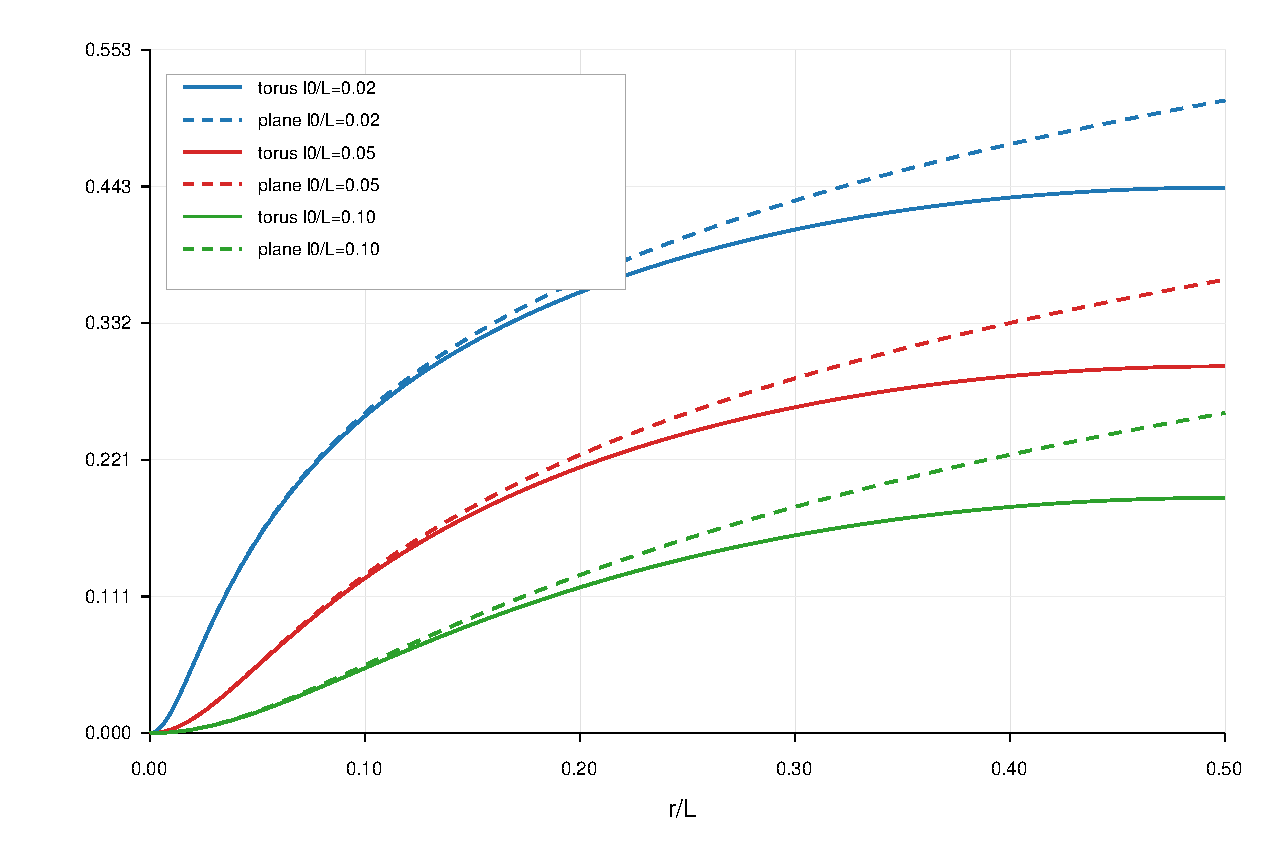
\includegraphics[width=0.5\linewidth]{torus_potential.pdf}
\caption{Axial finite-volume T-duality potential \eqref{axU} on the square torus. The solid curves show the zero-mode-subtracted toroidal pair energy \(\mathcal U_{\rm ax}(\xi;\mathfrak a)=\Delta V_{L,\ell_0}(r,0)/Q^2\) as a function of \(\xi=r/L\), for \(\mathfrak a=\ell_0/L\in\{0.02,0.05,0.10\}\). The dashed curves show the corrected infinite-plane reference potential \eqref{Uinf}. At small separations, the toroidal result approaches the infinite-plane potential, while at separations of order \(L\), the finite geometry and zero-mode subtraction produce a bounded periodic interaction.}
\label{fig:torus-potential}
\end{figure}

\begin{table}[t]
\caption{Convergence of the truncated square-torus mode sum used in Fig.~\ref{fig:torus-potential}. The cutoff \(N\) means \(-N\leq n_1,n_2\leq N\), with the zero mode omitted. The tail estimate is \(K_0(2\pi\mathfrak a N)/\pi\). The last column gives the direct convergence check on the plotting grid.}
\label{tab:torus-convergence}
\begin{ruledtabular}
\begin{tabular}{cccc}
\(\mathfrak a=\ell_0/L\) &
\(N\) &
\(K_0(2\pi\mathfrak a N)/\pi\) &
\(\displaystyle{\max_{0\leq\xi\leq 1/2}} |\mathcal U_{2N}-\mathcal U_N|\) \\
\hline
\(0.020\) & \(164\) & \(9.79\times10^{-11}\) & \(2.13\times10^{-11}\) \\
\(0.050\) & \(66\)  & \(8.61\times10^{-11}\) & \(1.73\times10^{-11}\) \\
\(0.100\) & \(33\)  & \(8.61\times10^{-11}\) & \(1.45\times10^{-11}\) \\
\end{tabular}
\end{ruledtabular}
\end{table}

For the numerical evaluation of the axial torus potential, we truncate the lattice sum symmetrically,
\begin{equation}
\mathcal U_N(\xi;\mathfrak a)=\sum_{\substack{-N\leq n_1,n_2\leq N\\(n_1,n_2)\neq(0,0)}}
\frac{\mathfrak a K_1(2\pi\mathfrak a|\mathbf n|)}{2\pi|\mathbf n|}
\left[1-\cos(2\pi n_1\xi)\right].
\end{equation}
For every fixed \(\mathfrak a>0\), this sum is exponentially convergent. The effective damping scale in the lattice sum is set by \(2\pi\mathfrak a|\mathbf n|\), and smaller values of \(\mathfrak a\) therefore require larger mode cutoffs. A useful estimate of the neglected tail is obtained by replacing the remaining lattice modes by a radial continuum integral. Using \(0\leq1-\cos(2\pi n_1\xi)\leq2\), one finds
\begin{equation}
  |R_N(\xi;\mathfrak a)|\lesssim2\mathfrak a\int_N^\infty d\rho\,K_1(2\pi\mathfrak a\rho)
  =\frac{1}{\pi}K_0(2\pi\mathfrak a N).
\end{equation}
We therefore choose \(N\) such that
\begin{equation}\label{cutoff}
  \frac{1}{\pi}K_0(2\pi\mathfrak a N)<10^{-10}.
\end{equation}
As an independent numerical check, we also compute
\begin{equation}\label{error}
\epsilon_N=\max_{\xi\in[0,1/2]}\left|\mathcal U_{2N}(\xi;\mathfrak a)-\mathcal U_N(\xi;\mathfrak a)\right|
\end{equation}
on the plotting grid. The values used in Fig.~\ref{fig:torus-potential} are shown in Table~\ref{tab:torus-convergence}. In all cases, the direct difference between the \(N\) and \(2N\) truncations is below \(2.2\times10^{-11}\), so the visible deviations between the toroidal curves and the infinite-plane reference are finite-size effects rather than truncation artefacts. The values in Table~\ref{tab:torus-convergence} scale approximately as \(N\propto1/\mathfrak a\), as expected from the exponential factor \(e^{-2\pi\mathfrak a|\mathbf n|}\). Fig.~\ref{fig:torus-potential} illustrates the separation between ultraviolet and infrared physics. At small \(\xi=r/L\), with \(s=r/\ell_0=\xi/\mathfrak a\) fixed and the charge far from its periodic images, the toroidal curves follow the corrected infinite-plane curve \eqref{Uinf}, in agreement with Proposition~\ref{prop:square-torus-zero-mode}. At larger separations, they bend away from the infinite-plane logarithm because the torus has no unbounded radial direction and the zero mode has been removed. The finite-volume potential is therefore a bounded periodic function, whereas the infinite-plane reference continues to grow logarithmically. The same limit gives the local small-distance regimes. For \(r\ll\ell_0\ll L\), one recovers the quadratic core found in the infinite plane,
\begin{equation}
  \Delta V_{L,\ell_0}(\mathbf r)=\frac{Q^2}{4\pi}\frac{r^2}{\ell_0^2}
  +\mathcal O\!\left(\frac{r^4}{\ell_0^4}\right)
  +\mathcal O\!\left(\frac{r^2}{L^2}\right).
\end{equation}
For \(\ell_0\ll r\ll L\), the logarithmic planar behavior is recovered,
\begin{equation}
\Delta V_{L,\ell_0}(\mathbf r)=\frac{Q^2}{2\pi}\ln\left(\frac{r}{\ell_0}\right)
+\mathcal O\!\left(\frac{\ell_0^2}{r^2}\right)
+\mathcal O\!\left(\frac{r^2}{L^2}\right).
\end{equation}
At separations comparable to \(L\), however, the potential is no longer described by an infinite-plane logarithm; it is a finite periodic function determined by the discrete spectrum of the torus. For numerical purposes, the direct Fourier series is efficient when \(2\pi\mathfrak a|\mathbf n|\) is not too small, because the T-duality factor suppresses large \(|\mathbf n|\) exponentially. When \(\mathfrak a\ll1\), an Ewald-type representation is preferable, as in standard treatments of periodic long-range Green functions \cite{Ewald1921,Linton1998}. Specialising the heat-kernel representation of Proposition~\ref{prop:spectral-td-green} to a neutral pair on the square torus gives
\begin{equation}
  \Delta V_{L,\ell_0}(\mathbf r)=Q^2\int_0^\infty ds\,e^{-s}\int_{\ell_0^2/(4s)}^\infty d\tau\,
  \left[K_{\mathbb T^2_L}(\tau;\mathbf 0)-K_{\mathbb T^2_L}(\tau;\mathbf r)\right],
\end{equation}
where
\begin{equation}
  K_{\mathbb T^2_L}(\tau;\mathbf r)=\frac{1}{L^2}\sum_{\mathbf n\in\mathbb Z^2}
  e^{-\tau k_{\mathbf n}^2}e^{i\mathbf k_{\mathbf n}\cdot\mathbf r}
\end{equation}
is the heat kernel on the square torus. By Poisson summation,
\begin{equation}
  K_{\mathbb T^2_L}(\tau;\mathbf r)=\frac{1}{4\pi\tau}\sum_{\mathbf m\in\mathbb Z^2}
  \exp\left(-\frac{|\mathbf r+L\mathbf m|^2}{4\tau}\right).
\end{equation}
The zero mode cancels in the difference \(K_{\mathbb T^2_L}(\tau;\mathbf 0)-K_{\mathbb T^2_L}(\tau;\mathbf r)\). This real-space representation makes explicit how the finite-volume result interpolates between the ultraviolet scale \(\ell_0\) and the infrared scale \(L\).


\subsection{Grounded half-plane}\label{subsec:half_plane}

We next consider Dirichlet boundary geometries, where the additive constant of the two-dimensional Green function is fixed by the grounded boundary condition. We begin with the upper half-plane
\(H=\{(x,y)\in\mathbb R^2:y>0\}\), with \(A_0(x,0)=0\). Let \(X=(x,y)\), \(X'=(x',y')\), and let \(X'_*=(x',-y')\) be the mirror point of \(X'\) across the boundary. The same heat-kernel argument also treats the strip \(S_W=\{(x,y)\in\mathbb R^2:0<y<W\}\), so it is useful to collect both image formulae in a single statement. The boundary image constructions used below are shown schematically in Fig.~\ref{fig:dirichlet-images}, which displays the half-plane mirror charge and the alternating image tower for the strip. 


\begin{proposition}\label{prop:dirichlet-images}
Let
\begin{equation}
  G_{\infty,\ell_0}^{\rm sub}(R)=-\frac{1}{4\pi}\ln\left(|R|^2+\ell_0^2\right),
\end{equation}
where the additive constant, or equivalently the reference length inside the logarithm, is immaterial in the differences below. For the upper half-plane \(H\),
\begin{equation}\label{GD}
  G_{H,\ell_0}^D(X,X')
  =G_{\infty,\ell_0}^{\rm sub}(X-X')-G_{\infty,\ell_0}^{\rm sub}(X-X'_*)
  =-\frac{1}{4\pi}\ln\left(\frac{|X-X'|^2+\ell_0^2}{|X-X'_*|^2+\ell_0^2}\right).
\end{equation}
In particular,
\begin{equation}
  G_{H,\ell_0}^D(X,X)=\frac{1}{4\pi}\ln\left(1+\frac{4y^2}{\ell_0^2}\right).
\end{equation}
For the strip \(S_W\), set
\begin{equation}
  \mathcal A=\sqrt{(x-x')^2+\ell_0^2}.
\end{equation}
The symmetrically summed alternating image series is
\begin{equation}
  G_{S_W,\ell_0}^D(X,X')=\sum_{p\in\mathbb Z}^{\rm sym}\left[
  G_{\infty,\ell_0}^{\rm sub}\bigl(x-x',y-y'+2pW\bigr)
  -G_{\infty,\ell_0}^{\rm sub}\bigl(x-x',y+y'+2pW\bigr)
  \right],
\end{equation}
which has the closed form
\begin{equation}\label{GFs}
  G_{S_W,\ell_0}^D(X,X')=-\frac{1}{4\pi}\ln\left[
  \frac{\cosh(\pi\mathcal A/W)-\cos\bigl(\pi(y-y')/W\bigr)}
  {\cosh(\pi\mathcal A/W)-\cos\bigl(\pi(y+y')/W\bigr)}\right].
\end{equation}
Its diagonal is finite and equals
\begin{equation}
  G_{S_W,\ell_0}^D(X,X)=\frac{1}{4\pi}\ln\left[
  \frac{\cosh(\pi\ell_0/W)-\cos(2\pi y/W)}{\cosh(\pi\ell_0/W)-1}\right].
\end{equation}
For \(X\neq X'\), the limits \(\ell_0\to0^+\) recover the ordinary Dirichlet Green functions.
\end{proposition}

\begin{proof}
The Dirichlet heat kernel on the half-plane is the antisymmetrisation
\begin{equation}
  K_H^D(\tau;X,X')=K_{\mathbb R^2}(\tau;X-X')-K_{\mathbb R^2}(\tau;X-X'_*).
\end{equation}
Since the T-duality kernel is obtained from the Dirichlet Laplacian by spectral functional calculus, equivalently by the heat-kernel representation of Proposition~\ref{prop:spectral-td-green}, the same antisymmetrisation applies after the T-duality smearing. Inserting the subtracted infinite-plane kernel gives \eqref{GD}, and setting \(X=X'\) gives the stated half-plane diagonal. For the strip, the Dirichlet heat kernel is the alternating tower over the images at \(y-y'+2pW\) and \(y+y'+2pW\). The same heat-kernel representation therefore gives the symmetrically summed image series. With \(b=y-y'\) and \(c=y+y'\), the Weierstrass product identity
\begin{equation}
  \prod_{p\in\mathbb Z}^{\rm sym}
  \frac{\mathcal A^2+(b+2pW)^2}{\mathcal A^2+(c+2pW)^2}
  =\frac{\cosh(\pi\mathcal A/W)-\cos(\pi b/W)}
  {\cosh(\pi\mathcal A/W)-\cos(\pi c/W)}
\end{equation}
then gives \eqref{GFs}; this is the standard product form underlying the strip Green function \cite{DLMF}. The diagonal follows by putting \(x=x'\) and \(y=y'\). Finally, for distinct points, \(\ell_0\to0^+\) sends \(\mathcal A\) to \(|x-x'|\) and recovers the local Dirichlet kernels.
\end{proof}

Equation~\eqref{GD} immediately satisfies the grounded boundary condition: if \(X\) lies on \(y=0\), then \(|X-X'|=|X-X'_*|\), and hence \(G_{H,\ell_0}^D((x,0),X')=0\). In the local limit one obtains
\begin{equation}
  G_{H,0}^D(X,X')=-\frac{1}{2\pi}\ln\left(\frac{|X-X'|}{|X-X'_*|}\right),
\end{equation}
as expected from the ordinary method of images \cite{Jackson1999}. Applying the local Laplacian to \eqref{GD} gives the boundary-adapted smeared source equation
\begin{equation}
  -\nabla_X^2G_{H,\ell_0}^D(X,X')=\rho_{\infty,\ell_0}(X-X')-\rho_{\infty,\ell_0}(X-X'_*),
\end{equation}
where
\begin{equation}
  \rho_{\infty,\ell_0}(R)=\frac{1}{\pi\ell_0^2}\left(1+\frac{|R|^2}{\ell_0^2}\right)^{-2}.
\end{equation}
Thus the boundary problem is not obtained by simply cutting off the infinite-plane charge cloud at \(y=0\). The spectral Dirichlet construction produces a boundary-compatible smeared source through antisymmetrisation. For a neutral pair with charges \(+Q\) and \(-Q\) at \(X_1\) and \(X_2\), the grounded half-plane energy is
\begin{equation}
  E_H^{(+,-)}=\frac{Q^2}{2}\left[G_{H,\ell_0}^D(X_1,X_1)+G_{H,\ell_0}^D(X_2,X_2)-2G_{H,\ell_0}^D(X_1,X_2)\right].
\end{equation}
Writing \(X_{2*}\) for the image of \(X_2\), this becomes
\begin{equation}
  E_H^{(+,-)}=\frac{Q^2}{8\pi}\ln\left(1+\frac{4y_1^2}{\ell_0^2}\right)
  +\frac{Q^2}{8\pi}\ln\left(1+\frac{4y_2^2}{\ell_0^2}\right)
  +\frac{Q^2}{4\pi}\ln\left(\frac{|X_1-X_2|^2+\ell_0^2}{|X_1-X_{2*}|^2+\ell_0^2}\right).
\end{equation}
This formula separates the two boundary self-energies from the direct charge-anticharge interaction, which is modified by the image geometry. The fact that the image construction works here is not automatic in arbitrary nonlocal electrodynamics. It follows from the spectral definition: the nonlocal operator is a function of the Dirichlet Laplacian, so it preserves the heat-kernel antisymmetrisation. For other nonlocal kernels or other boundary prescriptions, the ordinary image method can fail \cite{BorgesBufalo2025}.

\subsection{Grounded strip}\label{subsec:strip}

As a second boundary example, we consider the infinite strip \(S_W=\{(x,y)\in\mathbb R^2:0<y<W\}\), with grounded boundaries \(A_0(x,0)=A_0(x,W)=0\). The Dirichlet eigenfunctions are plane waves along the strip and standing waves in the transverse direction,
\begin{equation}
  u_{km}(x,y)=\frac{1}{\sqrt{\pi W}}\,e^{ikx}\sin\left(\frac{m\pi y}{W}\right),\qquad m=1,2,\ldots,
\end{equation}
with eigenvalues
\begin{equation}
  \lambda_{km}=k^2+\left(\frac{m\pi}{W}\right)^2.
\end{equation}
The spectral T-duality Green function is therefore
\begin{equation}
  G_{S_W,\ell_0}^D(X,X')=\frac{2}{W}\sum_{m=1}^{\infty}\sin\left(\frac{m\pi y}{W}\right)
  \sin\left(\frac{m\pi y'}{W}\right)
  \int_{-\infty}^{\infty}\frac{dk}{2\pi}\,
  \frac{\ell_0\sqrt{k^2+(m\pi/W)^2}K_1\!\left(\ell_0\sqrt{k^2+(m\pi/W)^2}\right)}{k^2+(m\pi/W)^2}
  e^{ik(x-x')}.
\end{equation}
This representation is exact and follows directly from the spectral definition. It is often the most convenient starting point for numerical evaluation. Proposition~\ref{prop:dirichlet-images} gives the equivalent image representation and its closed form \eqref{GFs}. The equivalence is a useful consistency check: the image method survives the nonlocal deformation precisely because the deformation is defined as a spectral function of the Dirichlet Laplacian. The closed form \eqref{GFs} satisfies both grounded boundary conditions,
\begin{equation}
  G_{S_W,\ell_0}^D((x,0),X')=G_{S_W,\ell_0}^D((x,W),X')=0.
\end{equation}
For \(X\neq X'\), its local limit is the usual Dirichlet Green function in an infinite strip,
\begin{equation}
  G_{S_W,0}^D(X,X')=-\frac{1}{4\pi}\ln\left[
  \frac{\cosh(\pi|x-x'|/W)-\cos\bigl(\pi(y-y')/W\bigr)}
  {\cosh(\pi|x-x'|/W)-\cos\bigl(\pi(y+y')/W\bigr)}\right].
\end{equation}
The diagonal of the local two-dimensional Green function is, of course, divergent; the finite diagonal in Proposition~\ref{prop:dirichlet-images} is the T-duality-regularised quantity. In the limit \(W\to\infty\), with \(y\) and \(y'\) fixed, the strip result reduces to the grounded half-plane expression,
\begin{equation}
  G_{S_W,\ell_0}^D(X,X')\longrightarrow
  -\frac{1}{4\pi}\ln\left(\frac{|X-X'|^2+\ell_0^2}{|X-X'_*|^2+\ell_0^2}\right).
\end{equation}
For a neutral pair in the strip, the energy is obtained from the same finite quadratic form,
\begin{equation}
  E_{S_W}^{(+,-)}=\frac{Q^2}{2}\left[G_{S_W,\ell_0}^D(X_1,X_1)+G_{S_W,\ell_0}^D(X_2,X_2)-2G_{S_W,\ell_0}^D(X_1,X_2)\right].
\end{equation}
This expression is finite without any additional ultraviolet subtraction. The finite zero-point length regularises the coincident limit, while the grounded boundaries remove the logarithmic infrared ambiguity.

\begin{corollary}\label{cor:boundary-self-forces}
The T-duality-regularised self-energy of a charge \(Q\) at height \(y\) above the grounded half-plane boundary is
\begin{equation}
  U_H^{\rm self}(y)=\frac{Q^2}{2}G_{H,\ell_0}^D(X,X)
  =\frac{Q^2}{8\pi}\ln\left(1+\frac{4y^2}{\ell_0^2}\right),
\end{equation}
and the corresponding normal force is
\begin{equation}
  F_y^H(y)=-\frac{dU_H^{\rm self}}{dy}
  =-\frac{Q^2y}{\pi(\ell_0^2+4y^2)}.
\end{equation}
In the grounded strip,
\begin{equation}
  U_{S_W}^{\rm self}(y)=\frac{Q^2}{8\pi}\ln\left[
  \frac{\cosh(\pi\ell_0/W)-\cos(2\pi y/W)}{\cosh(\pi\ell_0/W)-1}\right],
\end{equation}
and therefore
\begin{equation}
  F_y^{S_W}(y)=-\frac{dU_{S_W}^{\rm self}}{dy}
  =-\frac{Q^2}{4W}\,
  \frac{\sin(2\pi y/W)}{\cosh(\pi\ell_0/W)-\cos(2\pi y/W)}.
\end{equation}
Thus the strip force vanishes at the centre \(y=W/2\), points toward the nearer grounded wall, and is smoothed near each boundary by \(\ell_0\).
\end{corollary}

\begin{proof}
The half-plane and strip self-energies are \((Q^2/2)G^D(X,X)\), with the diagonal kernels supplied by Proposition~\ref{prop:dirichlet-images}. Differentiating the half-plane expression gives \(F_y^H\). For the strip,
\begin{equation}
  \frac{d}{dy}\left[\cosh(\pi\ell_0/W)-\cos(2\pi y/W)\right]
  =\frac{2\pi}{W}\sin(2\pi y/W),
\end{equation}
and the factor \((Q^2/8\pi)(2\pi/W)=Q^2/(4W)\) gives the stated force. Its sign changes across \(y=W/2\), where \(\sin(2\pi y/W)=0\).
\end{proof}

The half-plane force behaves as
\begin{equation}
  F_y^H=-\frac{Q^2}{\pi\ell_0^2}y+\mathcal O(y^3),\qquad y\ll\ell_0,
\end{equation}
near the boundary, so the zero-point length replaces the singular image-force onset by a linear restoring force. Far from the boundary,
\begin{equation}
  F_y^H=-\frac{Q^2}{4\pi y}+\mathcal O\!\left(\frac{\ell_0^2}{y^3}\right),\qquad y\gg\ell_0,
\end{equation}
which is the ordinary logarithmic two-dimensional image-force behavior. In the strip, the force is antisymmetric about the centre and vanishes at \(y=W/2\); near either grounded wall it is again smoothed by the nonzero length \(\ell_0\).

\begin{figure}[t]
\centering
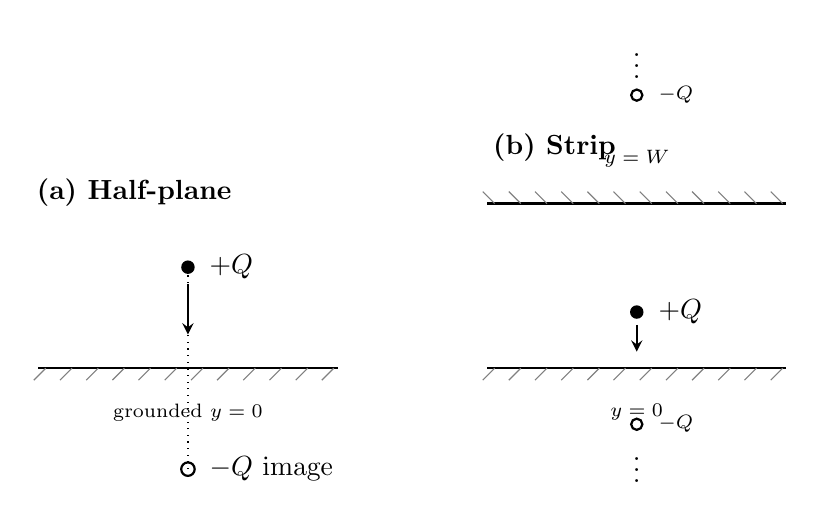
\begin{tikzpicture}[scale=0.95,>=stealth]
  \begin{scope}
    \node[anchor=west,font=\bfseries] at (-2.15,2.35) {(a) Half-plane};
    \draw[thick] (-2.0,0) -- (2.0,0);
    \foreach \x in {-1.9,-1.55,...,1.95} {\draw[gray] (\x,0) -- +( -0.16,-0.16);}
    \node[below] at (0,-0.35) {\scriptsize grounded $y=0$};
    \fill (0,1.35) circle (0.09);
    \node[right] at (0.16,1.35) {$+Q$};
    \draw[thick] (0,-1.35) circle (0.09);
    \node[right] at (0.16,-1.35) {$-Q$ image};
    \draw[dotted] (0,-1.35) -- (0,1.35);
    \draw[->,thick] (0,1.12) -- (0,0.45);
  \end{scope}
  \begin{scope}[xshift=6.0cm]
    \node[anchor=west,font=\bfseries] at (-2.05,2.95) {(b) Strip};
    \draw[thick] (-2.0,0) -- (2.0,0);
    \draw[thick] (-2.0,2.2) -- (2.0,2.2);
    \foreach \x in {-1.9,-1.55,...,1.95} {\draw[gray] (\x,0) -- +( -0.16,-0.16);}
    \foreach \x in {-1.9,-1.55,...,1.95} {\draw[gray] (\x,2.2) -- +( -0.16,0.16);}
    \node[below] at (0,-0.35) {\scriptsize $y=0$};
    \node[above] at (0,2.55) {\scriptsize $y=W$};
    \fill (0,0.75) circle (0.09);
    \node[right] at (0.16,0.75) {$+Q$};
    \draw[thick] (0,-0.75) circle (0.075);
    \node[right] at (0.16,-0.75) {\scriptsize $-Q$};
    \draw[thick] (0,3.65) circle (0.075);
    \node[right] at (0.16,3.65) {\scriptsize $-Q$};
    \node at (0,-1.25) {$\vdots$};
    \node at (0,4.15) {$\vdots$};
    \draw[->,thick] (0,0.58) -- (0,0.22);
  \end{scope}
\end{tikzpicture}
\caption{Image construction behind Proposition~\ref{prop:dirichlet-images}. In the half-plane a single mirror charge enforces the grounded boundary. In the strip the Dirichlet kernel is generated by an infinite alternating tower of images at \(\pm y+2pW\). The arrows indicate the direction of the boundary self-force described in Corollary~\ref{cor:boundary-self-forces}. The zero-point length \(\ell_0\) smooths the force near the grounded walls.}
\label{fig:dirichlet-images}
\end{figure}
The torus, half-plane, and strip illustrate complementary aspects of the same spectral construction. The torus preserves translational invariance but requires zero-mode subtraction. The grounded half-plane fixes the additive constant through a boundary condition and produces a finite image interaction. The strip combines two boundaries and admits both a spectral mode expansion and a closed image-summed expression. In all cases, the ultraviolet behavior is controlled by \(\ell_0\), whereas the infrared behavior is determined by the geometry.

\section{Running interaction dimension in finite volume}
\label{sec:running_dimension}

The preceding sections show that the T-duality scale $\ell_0$ regularises the ultraviolet behavior of the planar static Green function, whereas finite volume or boundary conditions regulate the infrared sector. It is therefore natural to ask how the associated {\it{running dimension}} behaves once both effects are included. In this section, we define an additive constant-free dimension diagnostic from the neutral-pair energy and evaluate it for the infinite plane, the square torus, the grounded half-plane, and the grounded strip. The notion of scale-dependent dimension is common in quantum gravity contexts, especially in analyses based on spectral dimension and diffusion processes  \cite{AmbjornJurkiewiczLoll2005, Benedetti2009, Horava2009, ModestoNicolini2010, Carlip2019, Calcagni2017}. The diagnostic used here is different. It is not a spectral dimension of an auxiliary random walk. It is an interaction dimension extracted from the scaling of an electrostatic observable. This distinction is important because different probes of a nonlocal or quantum geometry need not define the same scale-dependent dimension. Our goal is therefore not to identify a unique geometric dimension, but to quantify how the static interaction interpolates between its short-distance T-duality core and its infrared finite-volume behavior.  We also stress that the quantity introduced below is an operational interaction dimension. It measures the local logarithmic response of a static neutral-pair energy under a change of separation. It is not the spectral dimension of a diffusion process on $\Omega$, nor is it meant to define a unique intrinsic or fractal dimension of the underlying space. Different probes of a nonlocal theory can define different scale-dependent dimensions. The purpose of $\mathbb D_\Delta$ and $\mathbb D_F$ is narrower, i.e. they quantify how the T-duality-modified electrostatic interaction crosses over from its ultraviolet regularised core to the geometry-controlled infrared regime. For a neutral pair with charges $+Q$ and $-Q$ at $x$ and $x'$, the natural finite observable is
\begin{equation}
  \Delta V_\Omega(x,x')=\frac{Q^2}{2}\left[G_{\Omega,\ell_0}(x,x)+G_{\Omega,\ell_0}(x',x') - 2G_{\Omega,\ell_0}(x,x')\right].
\end{equation}
This quantity is invariant under the shift
\begin{equation}
  G_{\Omega,\ell_0}(x,x')\longrightarrow G_{\Omega,\ell_0}(x,x')+C,
\end{equation}
because the total charge of the pair is zero. Thus, it avoids the additive infrared ambiguity of the two-dimensional Green function. If the two points are varied along a one-parameter path with separation $r$, we define $\mathcal{V}_\Omega(r):=\Delta V_\Omega(r)/Q^2$. The potential-based running interaction dimension is then
\begin{equation}
  \mathbb D_\Delta(r)=3-\frac{\partial\ln \mathcal V_\Omega(r)}{\partial\ln r}.
\end{equation}
This definition is the finite-observable analogue of the potential-scaling definition used in previous work on T-duality electrodynamics \cite{GaeteNicolini2022, GaeteNicolini2026}. The difference is that the quantity entering the logarithm is now an unambiguous neutral-pair energy, rather than a Green function defined only up to an additive constant. A complementary diagnostic can be defined by the force
\begin{equation}
  \mathcal F_\Omega(r)=\frac{\partial\mathcal V_\Omega(r)}{\partial r},
\end{equation}
as
\begin{equation}
\mathbb D_F(r)=2-\frac{\partial\ln|\mathcal F_\Omega(r)|}{\partial\ln r}.
\end{equation}
For ordinary planar electrostatics, one has $\mathcal F(r)\propto r^{-1}$, and hence $\mathbb D_F=3$, the topological spacetime dimension. The force-based definition is also insensitive to additive constants, but in finite geometries, it becomes singular at points where the force vanishes. For this reason, $\mathbb D_\Delta$ is the better global diagnostic in finite volume, while $\mathbb D_F$ is useful locally on monotonic branches of the potential.

\subsection{Infinite-plane reference limit}
\label{subsec:running_dimension_infinite}

The corrected infinite-plane neutral-pair energy is
\begin{equation}
  \mathcal V_\infty(r)=\frac{1}{4\pi}\ln\left(1+\frac{r^2}{\ell_0^2}\right).
\end{equation}
Introducing $s=r/\ell_0$, we find
\begin{equation}
  \frac{\partial\ln \mathcal V_\infty}{\partial\ln r}=\frac{2s^2}{(1+s^2)\ln(1+s^2)}.
\end{equation}
Therefore
\begin{equation}\label{Dinf}
  \mathbb D_\Delta^{(\infty)}(s)=3-\frac{2s^2}{(1+s^2)\ln(1+s^2)}.
\end{equation}
At a short distance,
\begin{equation}
  \mathbb D_\Delta^{(\infty)}(s)=1+s^2-\frac{5}{6}s^4+\mathcal{O}(s^6),\qquad s\ll 1.
\end{equation}
Thus, the interaction probes an effective one-dimensional ultraviolet scaling. At large distance,
\begin{equation}
  \mathbb D_\Delta^{(\infty)}(s)=3-\frac{1}{\ln s}+\mathcal{O}\!\left(\frac{1}{s^2\ln s}\right),\qquad s\gg 1,
\end{equation}
so the classical value is recovered only logarithmically slowly. The force-based diagnostic gives a slightly different interpolation. Since
\begin{equation}
\mathcal F_\infty(r)=\frac{1}{2\pi}\frac{r}{r^2+\ell_0^2},
\end{equation}
one obtains
\begin{equation}
\mathbb D_F^{(\infty)}(s)=2-\frac{\partial}{\partial\ln s}\ln\left(\frac{s}{1+s^2}\right)
=\frac{1+3s^2}{1+s^2}.
\end{equation}
Thus $\mathbb D_F^{(\infty)}(0)=1$, and $\mathbb D_F^{(\infty)}(\infty)=3$. The limiting values agree with the potential-based definition, although the interpolation is different. This illustrates why the running dimension used here should be read as an operational interaction diagnostic rather than an intrinsic geometric dimension.

\subsection{Square torus}
\label{subsec:running_dimension_torus}

For the square torus, the neutral-pair energy is given by \eqref{DVT}. We also recall that by writing $\mathfrak{a}=\ell_0/L$, and $\boldsymbol{\xi}=\mathbf r/L$, we can define the dimensionless energy as
\begin{equation}
  \mathcal U_{\mathbb T^2}(\boldsymbol{\xi};\mathfrak{a})=\frac{\Delta V_{L,\ell_0}(\mathbf r)}{Q^2}=\sum_{\mathbf n\neq\mathbf 0}w_{\mathbf n}(\mathfrak{a})\left[1-\cos(2\pi\mathbf n\cdot\boldsymbol{\xi})\right],\quad w_{\mathbf n}(\mathfrak{a})=\frac{\mathfrak{a}K_1(2\pi \mathfrak{a}|\mathbf n|)}{2\pi|\mathbf n|}.
\end{equation}
Because the square torus is not rotationally invariant, the running dimension is path-dependent at separations comparable with $L$. Let $\boldsymbol{\xi}=\xi\hat e$, where $|\hat e|=1$, and define $q_{\mathbf n}(\hat e)=2\pi\,\mathbf n\cdot\hat e$. Then
\begin{equation}
  \mathcal U_{\hat e}(\xi;\mathfrak{a})=\sum_{\mathbf n\neq\mathbf 0}w_{\mathbf n}(\mathfrak{a})\left[1-\cos(q_{\mathbf n}\xi)\right].
\end{equation}
The potential-based running dimension along this path is
\begin{equation}\label{DDelta}
  \mathbb D_{\Delta,\mathbb T^2}(\xi;\mathfrak{a},\hat e)=3-\frac{\displaystyle\sum_{\mathbf n\neq\mathbf 0} w_{\mathbf n}(\mathfrak{a})\,q_{\mathbf n}\xi\,\sin(q_{\mathbf n}\xi)}{\displaystyle\sum_{\mathbf n\neq\mathbf 0}w_{\mathbf n}(\mathfrak{a})\left[1-\cos(q_{\mathbf n}\xi)\right]}.
\end{equation}
This expression is the appropriate quantity to plot as a function of $r/L=\xi$ for fixed $\ell_0/L=\mathfrak{a}$. The axial direction, $\hat e=(1,0)$ with $0\leq \xi\leq 1/2$, is a convenient canonical choice (see Fig.~\ref{fig:running-dimension-torus}). Notice that the ultraviolet limit is universal. Moreover, Fig.~\ref{fig:running-dimension-torus} shows the potential-based running interaction dimension along the axial direction of the square torus. The derivative entering $\mathbb D_\Delta$ is evaluated analytically from the truncated Fourier series, rather than by finite differences. Thus, if
\begin{equation}
  \mathcal U_{\rm ax}(\xi;\mathfrak a)=\sum_{\mathbf n\neq0} w_{\mathbf n}(\mathfrak a)\left[1-\cos(2\pi n_1\xi)\right],
\end{equation}
then
\begin{equation}
  \xi\,\partial_\xi\mathcal U_{\rm ax}(\xi;\mathfrak a) = \sum_{\mathbf n\neq0}w_{\mathbf n}(\mathfrak a)(2\pi n_1\xi)\sin(2\pi n_1\xi).
\end{equation}
At $\xi=0$, the plotted value is the limiting value $\mathbb D_\Delta= 1$. At the axial symmetry point $\xi=1/2$, periodicity implies $\partial_\xi\mathcal U_{\rm ax}=0$, and therefore $\mathbb D_\Delta=3$. Furthermore, Fig.~\ref{fig:running-dimension-torus} illustrates the distinction between ultraviolet and infrared behavior. The ultraviolet limit is controlled locally by the T-duality core and is insensitive to the global geometry because the neutral-pair energy is quadratic at small separation (see Eq.~\ref{smallxi}), so $\mathbb D_\Delta\to 1$. By contrast, the infrared behavior is geometry-dependent. The infinite-plane reference continues to approach the classical value $3$ only logarithmically, while the toroidal curves saturate at separations of order $L$ because the potential is bounded, periodic, and zero-mode subtracted.  The numerical convergence of the running-dimension curves is checked separately from the convergence of the potential. This is necessary because $\mathbb D_\Delta$ is a logarithmic derivative and therefore contains the ratio $\xi\,\partial_\xi\mathcal U_{\rm ax}/\mathcal U_{\rm ax}$. Although both numerator and denominator are smooth for $\mathfrak a>0$, they vanish as $\xi^2$ near the origin. In the plot, we therefore use the limiting value $\mathbb D_\Delta(0)=1$ at $\xi=0$, and evaluate the ratio only for $\xi>0$. The derivative is computed analytically from the truncated Fourier series, not by finite differences. Furthermore, the numerical evaluation of Fig.~\ref{fig:running-dimension-torus} uses the same symmetric lattice truncation as the toroidal potential. For each value of $\mathfrak a=\ell_0/L$, the cutoff $N$ is chosen according to \eqref{cutoff}. The running dimension is then computed from the analytic logarithmic derivative of the truncated sum. As a direct convergence check, the curve obtained with cutoff $N$ is compared with the curve obtained with cutoff $2N$ on the plotting grid, i.e.
\begin{equation}
  \epsilon_N^{(\mathbb D)}=\max_{\xi\in[0,1/2]}\left|\mathbb D_{\Delta,N}(\xi;\mathfrak a) -\mathbb D_{\Delta,2N}(\xi;\mathfrak a)\right|.
\end{equation}
The values are reported in Table~\ref{tab:running-dimension-convergence}. The direct $N$ versus $2N$ comparison is zero at the printed numerical precision for all three curves, confirming that the observed saturation of the toroidal running dimension is a finite-size effect rather than a truncation artifact.

Expanding at small $\xi$ gives
\begin{equation}\label{smallxi}
  \mathcal U_{\hat e}(\xi;\mathfrak{a})=A_2(\mathfrak{a},\hat e)\,\xi^2+A_4(\mathfrak{a},\hat e)\,\xi^4+\mathcal{O}(\xi^6),
\end{equation}
where
\begin{equation}
  A_2(\mathfrak{a},\hat e)=\frac{1}{2}\sum_{\mathbf n\neq\mathbf 0} w_{\mathbf n}(\mathfrak{a})q_{\mathbf n}^2,\quad  A_4(\mathfrak{a},\hat e)=-\frac{1}{24}\sum_{\mathbf n\neq\mathbf 0}w_{\mathbf n}(\mathfrak{a})q_{\mathbf n}^4.
\end{equation}
For every fixed $\mathfrak{a} > 0$, these sums are finite because the Bessel factor gives exponential suppression at large $|\mathbf n|$. Consequently,
\begin{equation}
  \frac{\partial\ln\mathcal U_{\hat e}}{\partial\ln\xi}=2+2\frac{A_4(\mathfrak{a},\hat e)}{A_2(\mathfrak{a},\hat e)}\xi^2+\mathcal{O}(\xi^4),
\end{equation}
and hence
\begin{equation}
  \mathbb D_{\Delta,\mathbb T^2}(\xi;\mathfrak{a},\hat e)=1+\kappa_{\mathbb T^2}(\mathfrak{a},\hat e)\xi^2+\mathcal{O}(\xi^4)
\end{equation}
with
\begin{equation}
  \kappa_{\mathbb T^2}(\mathfrak{a},\hat e)=\frac{1}{6}\frac{\displaystyle\sum_{\mathbf n\neq\mathbf 0}w_{\mathbf n}(\mathfrak{a})q_{\mathbf n}^4}{\displaystyle\sum_{\mathbf n\neq\mathbf 0}w_{\mathbf n}(\mathfrak{a})q_{\mathbf n}^2}.
\end{equation}
Thus
\begin{equation}
  \lim_{\xi\to 0}\mathbb D_{\Delta,\mathbb T^2}(\xi;\mathfrak{a},\hat e)=1. 
\end{equation}
The ultraviolet dimensional reduction is therefore not an artefact of the infinite plane. It survives finite volume because it is controlled by the local quadratic core of the T-duality-regularised potential. The large-volume limit reproduces the infinite-plane result. If $\mathfrak{a}\to 0$, $\xi\to 0$, and $s=\xi/\mathfrak{a}=r/\ell_0$ fixed, the toroidal sum approaches the continuum integral and $\mathcal U_{\hat e}(\xi;\mathfrak{a})\longrightarrow(4\pi)^{-1}\ln(1+s^2)$. As a consequence, $\mathbb D_{\Delta,\mathbb T^2}(\xi;\mathfrak{a},\hat e)\longrightarrow\mathbb D_\Delta^{(\infty)}(s)$. The infrared behavior is qualitatively different from that of the infinite plane. On the torus, there is no limit $r\to\infty$. The largest inequivalent separations are of order $L$. The potential is bounded, periodic, and smooth. For the axial path, periodicity implies $\mathcal U_{\rm ax}(\xi;\mathfrak{a})=\mathcal U_{\rm ax}(1-\xi;\mathfrak{a})$, so
\begin{equation}
  \left.\frac{\partial\mathcal U_{\rm ax}}{\partial\xi}\right|_{\xi=1/2}=0.
\end{equation}
Since $\mathcal U_{\rm ax}(1/2;\mathfrak{a})$ is finite and nonzero, the running dimension saturates at
\begin{equation}
  \mathbb D_{\Delta,\mathbb T^2}(1/2;\mathfrak{a},\hat x)=3.
\end{equation}

\begin{figure}[t]
    \centering
    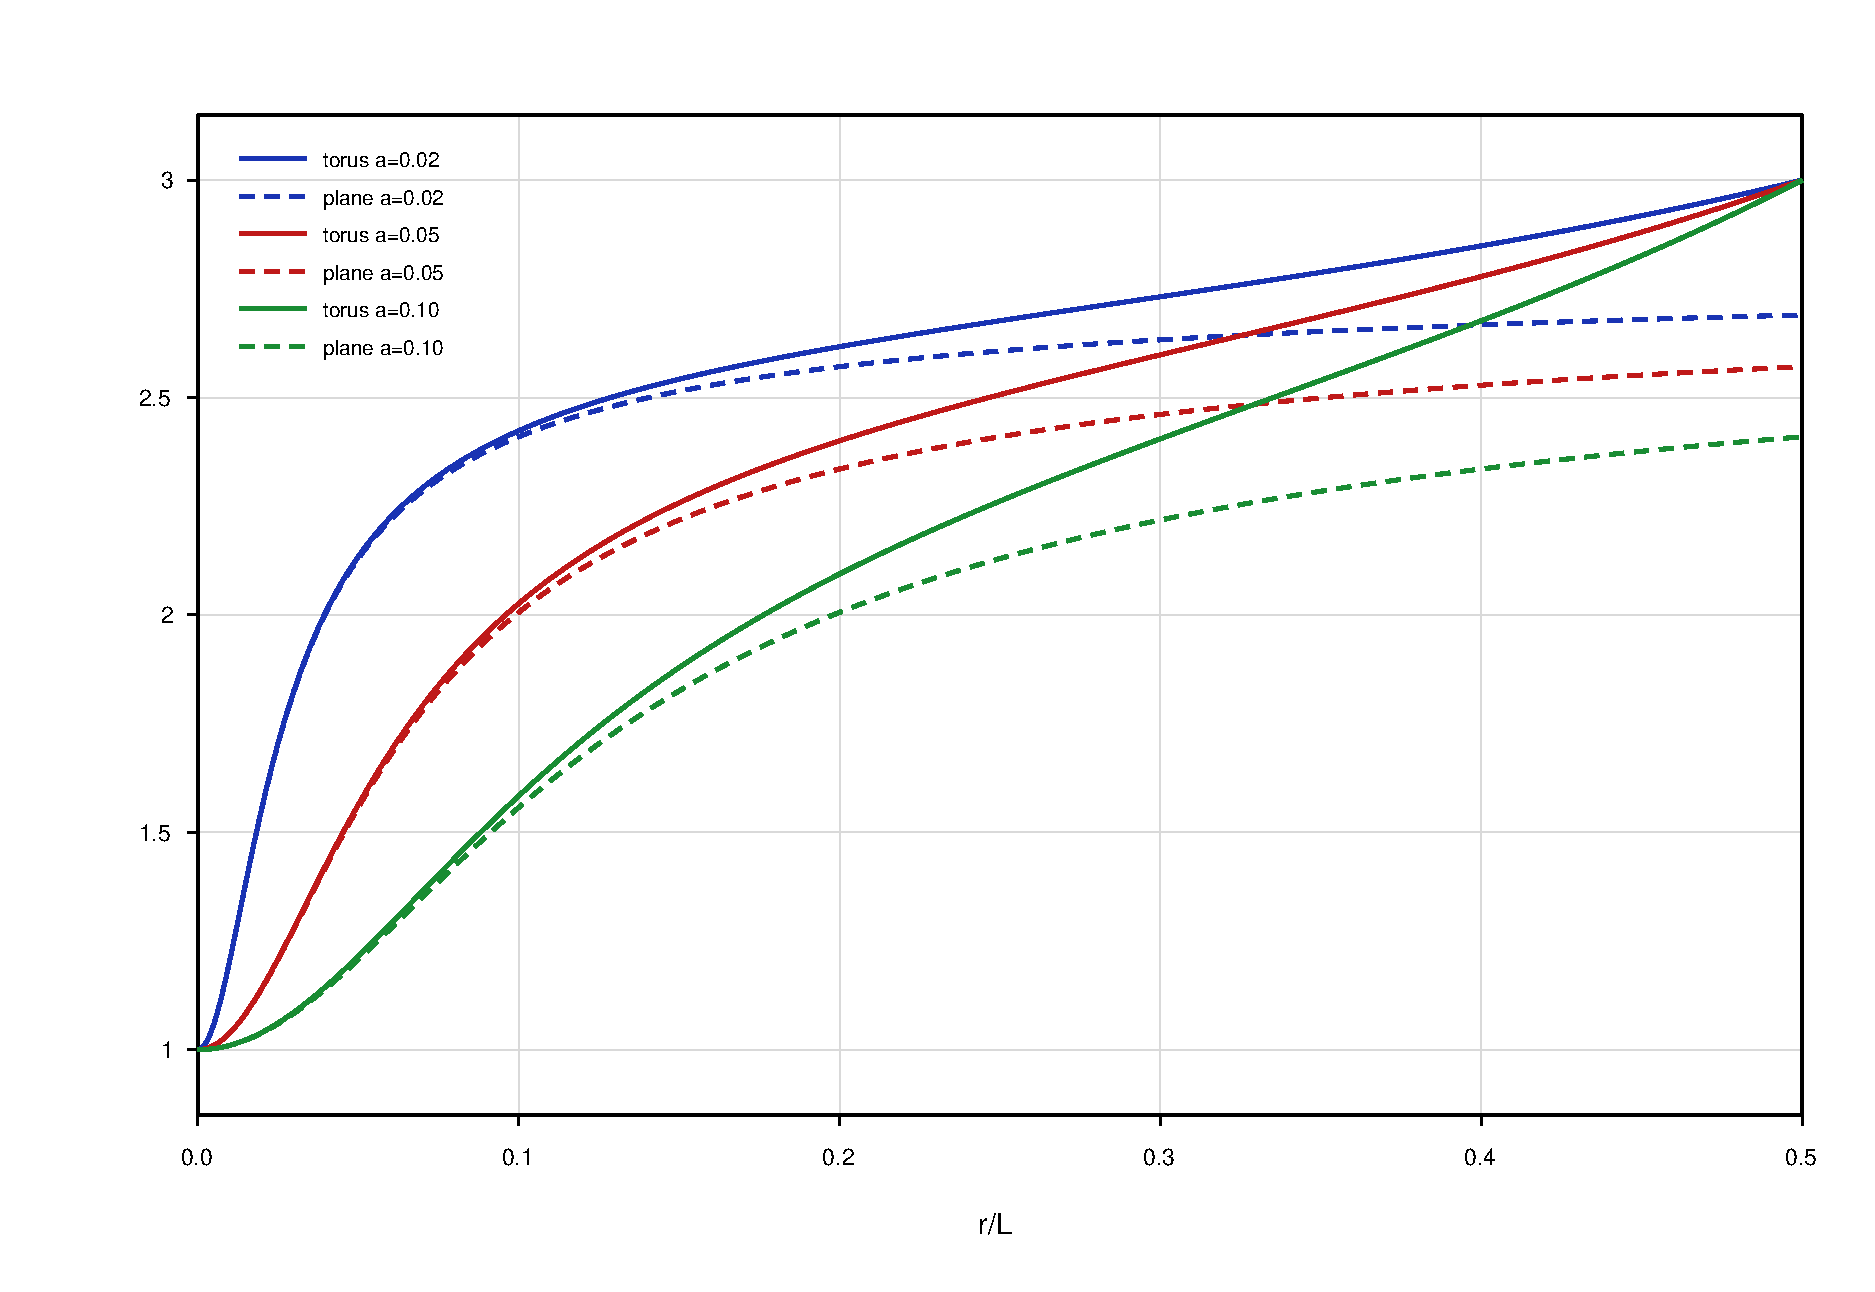
\includegraphics[width=0.5\linewidth]{running_dimension_torus.pdf}
    \caption{Potential-based running interaction dimension for the corrected infinite plane and for the square torus. The horizontal axis is $\xi=r/L$, and $\mathfrak a=\ell_0/L$. Solid curves show the toroidal result $\mathbb D_{\Delta,\mathbb T^2}(\xi;\mathfrak a,\hat x)$ obtained from the zero-mode-subtracted axial mode sum (see Eq.~\eqref{DDelta}), while dashed curves show the corrected infinite-plane reference $\mathbb D_\Delta^{(\infty)}(\xi/\mathfrak a)$. All curves approach the ultraviolet limit $\mathbb D_\Delta\to 1$ as $\xi\to 0$. The finite-torus curves saturate to $\mathbb D_\Delta=3$ at the maximally separated axial point $\xi=1/2$, where the potential is smooth and periodic, whereas the infinite-plane reference approaches $3$ only through the logarithmic large-distance limit.}
    \label{fig:running-dimension-torus}
\end{figure}

\begin{table}[t]
\caption{Convergence of the truncated square-torus mode sum used for the running-dimension plot in Fig.~\ref{fig:running-dimension-torus}. The cutoff $N$ means $-N\leq n_1,n_2\leq N$, with the zero mode omitted. The tail estimate is $K_0(2\pi\mathfrak a N)/\pi$. The last column gives the direct comparison between the curves computed with cutoffs $N$ and $2N$ on the plotting grid. The value $0.00$ in the last column means zero at the printed double-precision output of the convergence script.}
\label{tab:running-dimension-convergence}
\begin{ruledtabular}
\begin{tabular}{cccc}
$\mathfrak a=\ell_0/L$ &
$N$ &
$K_0(2\pi\mathfrak a N)/\pi$ &
$\max_\xi|\mathbb D_{\Delta,2N}-\mathbb D_{\Delta,N}|$ \\
\hline
$0.020$ & $328$ & $7.79\times10^{-20}$ & $0.00$ \\
$0.050$ & $132$ & $6.04\times10^{-20}$ & $0.00$ \\
$0.100$ & $66$  & $6.04\times10^{-20}$ & $0.00$ \\
\end{tabular}
\end{ruledtabular}
\end{table}

Thus, finite volume cuts off the logarithmic growth and replaces the infinite-plane slow approach to $3$ by a geometry-controlled saturation at the scale $r\sim L$. The force-based toroidal diagnostic is
\begin{equation}
  \mathbb D_{F,\mathbb T^2}(\xi;\mathfrak{a},\hat e)=2-\xi\frac{\displaystyle\sum_{\mathbf n\neq\mathbf 0}w_{\mathbf n}(\mathfrak{a})q_{\mathbf n}^2\cos(q_{\mathbf n}\xi)}{\displaystyle\sum_{\mathbf n\neq\mathbf 0}w_{\mathbf n}(\mathfrak{a})q_{\mathbf n}\sin(q_{\mathbf n}\xi)}.
\end{equation}
It again satisfies
\begin{equation}
  \lim_{\xi\to0}\mathbb D_{F,\mathbb T^2}(\xi;\mathfrak{a},\hat e)=1,
\end{equation}
but it becomes ill-defined at symmetry points where the force vanishes, such as $\xi=1/2$ along the axial path. This is why $\mathbb D_\Delta$ is the more robust finite-volume diagnostic.

\subsection{Grounded half-plane}
\label{subsec:running_dimension_halfplane}

The grounded half-plane is not finite in area, but the boundary fixes the additive constant and screens the neutral-pair energy at large separation parallel to the wall. Consider two charges at the same height $y>0$ above the grounded boundary, separated by a horizontal distance $R$, that is  $X_1=(0,y)$, and $X_2=(R,y)$. From the half-plane Green function \eqref{GD}, the neutral-pair energy is
\begin{equation}
  \Delta V_H(R;y)=Q^2\left[G_{H,\ell_0}^D(X_1,X_1)-G_{H,\ell_0}^D(X_1,X_2)\right].
\end{equation}
More precisely, we find
\begin{equation}
  \Delta V_H(R;y)=\frac{Q^2}{4\pi}h_H(\eta,b),
\end{equation}
where $\eta=R/\ell_0$, $b=(2y)/\ell_0$, and
\begin{equation}
  h_H(\eta,b)=\ln\left[\frac{(1+b^2)(1+\eta^2)}{1+b^2+\eta^2}\right].
\end{equation}
This function vanishes at $R=0$ and tends to a finite constant as $R\to\infty$, that is $h_H(0,b)=0$, and $h_H(\infty,b)=\ln(1+b^2)$. The corresponding running interaction dimension is
\begin{equation}
  \mathbb D_{\Delta,H}(\eta;b)=3-\frac{2\eta^2 b^2}{(1+\eta^2)(1+b^2+\eta^2)\ln\left[\frac{(1+b^2)(1+\eta^2)}{1+b^2+\eta^2}\right]}.
\end{equation}
At short horizontal separation, we have
\begin{equation}
  h_H(\eta,b)=\frac{b^2}{1+b^2}\eta^2+\mathcal{O}(\eta^4),\qquad\eta\ll 1,
\end{equation}
and therefore $\mathbb D_{\Delta,H}(\eta;b)=1+\mathcal{O}(\eta^2)$. The same ultraviolet dimensional reduction is recovered. At large horizontal separation,
\begin{equation}
h_H(\eta,b)=\ln(1+b^2)-\frac{b^2}{\eta^2}+\mathcal{O}(\eta^{-4}),\qquad\eta\gg 1,
\end{equation}
which gives
\begin{equation}
\mathbb D_{\Delta,H}(\eta;b)=3-\frac{2b^2}{\eta^2\ln(1+b^2)}+\mathcal{O}(\eta^{-4}).
\end{equation}
Thus, the interaction dimension approaches the classical value algebraically. The grounded boundary has removed the logarithmic infrared growth. Hence, the energy does not diverge, but saturates to the finite value
\begin{equation}
  \Delta V_H(\infty;y)=\frac{Q^2}{4\pi}\ln\left(1+\frac{4y^2}{\ell_0^2}\right).
\end{equation}

\subsection{Grounded strip}
\label{subsec:running_dimension_strip}

The grounded strip provides a fully confined transverse geometry and a stronger infrared cutoff. Consider the strip $0<y<W$ with Dirichlet boundary conditions at $y=0$ and $y=W$. We place the two charges at equal height $y$ and separate them by a distance $R$ along the strip, i.e. $X_1=(0,y)$, and $X_2=(R,y)$. Using the strip Green function \eqref{GFs} yields the following expression for the neutral-pair energy
\begin{equation}
  \Delta V_{S_W}(R;y)=Q^2\left[G_{S_W,\ell_0}^D(X_1,X_1)-G_{S_W,\ell_0}^D(X_1,X_2)\right].
\end{equation}
Let us introduce the dimensionless variables $u=R/W$, $\widehat{a}=\ell_0/W$, $v=y/W$, and define
\begin{equation}
  \alpha(u) = \pi\sqrt{u^2+\widehat{a}^2}, \qquad \alpha_0 = \pi \widehat{a},\qquad c_v = \cos(2\pi v).
\end{equation}
Then the neutral-pair energy becomes
\begin{equation}
  \Delta V_{S_W}(R;y)=\frac{Q^2}{4\pi}h_S(u;\widehat{a},v),\quad h_S(u;\widehat{a},v)=\ln\left[\frac{\cosh\alpha_0-c_v}{\cosh\alpha_0-1}\,\frac{\cosh\alpha(u)-1}{\cosh\alpha(u)-c_v}\right].
\end{equation}
with $h_S(0;\widehat{a},v)=0$, and
\begin{equation}
  h_S(\infty;\widehat{a},v):=\lim_{u\to\infty}h_S(u;\widehat{a},v)=\ln\left[\frac{\cosh(\pi \widehat{a})-\cos(2\pi v)}{\cosh(\pi \widehat{a})-1}\right].
\end{equation}
Thus, the energy saturates at large longitudinal separation. The logarithmic derivative is
\begin{equation}
  \frac{\partial h_S}{\partial\ln u}=\frac{\pi(1-c_v)u^2\sinh\alpha(u)}{\sqrt{u^2+\widehat{a}^2}[\cosh\alpha(u)-1][\cosh\alpha(u)-c_v]}.
\end{equation}
The strip running dimension is therefore
\begin{equation}
\mathbb D_{\Delta,S_W}(u;\widehat{a},v)=3-\frac{\pi(1-c_v)u^2\sinh\alpha(u)}{\sqrt{u^2+\widehat{a}^2}[\cosh\alpha(u)-1][\cosh\alpha(u)-c_v]\ln\left[\frac{\cosh\alpha_0-c_v}{\cosh\alpha_0-1}
\,\frac{\cosh\alpha(u)-1}{\cosh\alpha(u)-c_v}\right]}.
\end{equation}
At short separation,
\begin{equation}
h_S(u;\widehat{a},v)=C_2(\widehat{a},v)u^2+\mathcal{O}(u^4),\qquad u\ll1,
\end{equation}
with
\begin{equation}
C_2(\widehat{a},v)=\frac{\pi\sinh(\pi\widehat{a})}{2\widehat{a}}\left[
\frac{1}{\cosh(\pi \widehat{a})-1}-\frac{1}{\cosh(\pi\widehat{a})-\cos(2\pi v)}\right].
\end{equation}
Hence
\begin{equation}
\mathbb D_{\Delta,S_W}(u;\widehat{a},v)=1+\mathcal{O}(u^2),\qquad u\ll 1.
\end{equation}
The ultraviolet flow to one dimension again survives. At large longitudinal separation, $\alpha(u)=\pi u+\mathcal{O}(u^{-1})$ for $u\gg 1$, and the second factor in $h_S$ approaches unity exponentially. More precisely, we find
\begin{equation}
\frac{\cosh\alpha(u)-1}{\cosh\alpha(u)-c_v}=1-2(1-c_v)e^{-\alpha(u)}+\mathcal{O}(e^{-2\alpha(u)}).
\end{equation}
Therefore, 
\begin{equation}
h_S(u;\widehat{a},v)=h_S(\infty;\widehat{a},v)-2(1-c_v)e^{-\alpha(u)}+\mathcal{O}(e^{-2\alpha(u)}),
\end{equation}
and
\begin{equation}
\mathbb D_{\Delta,S_W}(u;\widehat{a},v)=3-\frac{2\pi(1-c_v)u^2}{\sqrt{u^2+\widehat{a}^2}h_S(\infty;\widehat{a},v)}~e^{-\alpha(u)}+\mathcal{O}\left(\frac{u^2 e^{-2\alpha(u)}}{\sqrt{u^2+\widehat{a}^2}}\right).
\end{equation}
Finally, using $\alpha(u)=\pi u+\mathcal{O}(u^{-1})$ and $u^2/\sqrt{u^2+\widehat{a}^2}=u+\mathcal{O}(u^{-1})$, we can further simplify the leading behavior and obtain the final result
\begin{equation}
\mathbb D_{\Delta,S_W}(u;\widehat{a},v)=3-\frac{2\pi(1-c_v)}{h_S(\infty;\widehat{a},v)}ue^{-\pi u}\left[1+\mathcal{O}(u^{-1})\right].
\end{equation}
The strip, therefore, reaches the classical value exponentially fast. The transverse gap $\pi/W$ replaces the infinite-plane logarithmic infrared tail by finite-size saturation. The results above can be summarised as follows. The ultraviolet limit is local and universal, i.e. $\mathcal V(r)\propto r^2$ implies $\mathbb D_\Delta(r)\to 1$. This follows from the finite T-duality core and is independent of the global geometry, provided the charge separation is small compared with both $\ell_0$ and the geometric infrared scale. By contrast, the infrared behavior is geometry-dependent. On the infinite plane, the potential grows logarithmically, and the running dimension approaches $3$ only as $1/\ln(r/\ell_0)$. On the torus, the potential is bounded and periodic, so the flow saturates at separations of order $L$. In the half-plane and strip, grounded boundaries screen the neutral-pair energy, whereas in the strip, the approach to saturation is exponential due to the transverse spectral gap. Thus, finite volume and boundary conditions do not destroy the short-distance dimensional reduction induced by the T-duality kernel. Instead, they replace the infrared logarithmic divergence of the infinite plane with a finite, geometry-controlled saturation.

\section{Conclusions and outlook}
\label{sec:conclusions}

We have developed a finite-size formulation of T-duality-deformed electrostatics in $(2+1)$ dimensions. The main point of the construction is that the zero-point length $\ell_0$ and the infrared geometry play logically distinct roles. The T-duality form factor $f(k)=\ell_0 kK_1(\ell_0 k)$ regularises the ultraviolet behavior of the static Green function, whereas the large-distance behavior is fixed by the spectrum, zero-mode prescription, and boundary conditions of the spatial domain. This separation is essential in two dimensions, where the ordinary Maxwell Green function is logarithmic and therefore carries an unavoidable additive infrared ambiguity. As a first step, we rederived the infinite-plane kernel in an explicitly subtracted form. Starting from the same static momentum-space propagator used in T-duality electrodynamics, the self-energy-subtracted neutral-pair interaction is given by \eqref{DeltaV}. This result is finite at the origin, grows quadratically for $r\ll\ell_0$, and recovers the ordinary logarithmic Coulomb interaction for $r\gg\ell_0$. The derivation also shows that the T-duality kernel may be interpreted as a local Poisson problem sourced by the normalised algebraic charge cloud \eqref{density}. This observation provides a useful physical interpretation of the ultraviolet regularisation: the point charge is replaced by a finite distribution with a radius set by $\ell_0$. The second result of the paper is a spectral formulation of the same nonlocal kernel on finite, bounded domains. If $A_B=-\Delta_B$ is a non-negative self-adjoint realization of the Laplacian on a domain $\Omega$, with eigenpairs $(\lambda_n,u_n)$, the T-duality Green operator is $\mathcal G_{\Omega,\ell_0}^{(B)}=F_{\ell_0}(A_B)A_B^{-1}P_\perp$ with $F_{\ell_0}(\lambda)=\ell_0\sqrt{\lambda}\, K_1(\ell_0\sqrt{\lambda})$, and its kernel is represented by \eqref{GB}. This definition is not a formal restriction of the infinite-plane convolution kernel. Rather, the boundary condition is imposed before the nonlocal function of the Laplacian is formed. Consequently, different self-adjoint realisations of $-\Delta$ define different nonlocal electrostatic theories. This is the natural framework when the T-duality correction is interpreted as a function of the kinetic operator itself, as in the spectral treatment of nonlocal and fractional elliptic operators \cite{Seeley1967, Grubb2015, Kwasnicki2017, BonitoPasciak2015}. The square torus gives the simplest finite-volume realisation. The constant mode must be removed, and this zero-mode subtraction is precisely equivalent to adding the uniform neutralising background required by charge neutrality on a compact space. For a neutral pair on $\mathbb T_L^2$, we obtained the exact positive mode sum represented by \eqref{DVT}. The exponential falloff of $K_1$ makes the ultraviolet convergence manifest, while the absence of the zero mode makes the infrared sector finite. In the limit $L\to\infty$, with $r$ and $\ell_0$ fixed, the toroidal result reduces to the corrected infinite-plane interaction above. For domains with boundaries, the spectral construction also gives explicit closed-form results. In the grounded half-plane, the Dirichlet heat kernel allows the image representation \eqref{GD} whose diagonal value is finite, and the boundary-induced force on a single charge is smoothed near the wall. Thus, the zero-point length not only regularises coincident charge interactions but also softens boundary self-forces. In the grounded strip, the same spectral construction admits both a transverse-mode expansion and a closed image-summed expression represented by \eqref{GFs}. That formula reduces to the standard Dirichlet strip Green function when $\ell_0\to 0$ and to the grounded half-plane result when $W\to\infty$. We also introduced an additive-constant-free running interaction dimension. The important point is that the diagnostic must be defined in terms of a physically neutral-pair observable, such as $\Delta V$, rather than an absolute two-dimensional Green function. For the infinite plane, the result is represented by \eqref{Dinf}. In that case, $\mathbb D_\Delta^{(\infty)}\to 1$ as $r\to 0$ and approaches the classical value $3$ only logarithmically at large distance. In finite volume and in bounded geometries, the ultraviolet limit remains universal, that is $\Delta V(r)\propto r^2$ implies $\mathbb D_\Delta(r)\to 1$. The infrared behavior, however, is not universal. On the torus, the flow saturates at separations of order $L$ because the potential is bounded and periodic. In the half-plane and strip, grounded boundaries screen the neutral-pair energy; in the strip, the approach to saturation is exponential, controlled by the transverse gap $\pi/W$. Thus, the short-distance dimensional reduction induced by the T-duality kernel survives finite volume, while the long-distance flow is determined by geometry. A useful by-product of the analysis is the clarification of the marginal infinite-plane limit. The corrected free-space result differs from the previously quoted expression for the same $(2+1)$-dimensional static kernel \cite{GaeteNicolini2026}. The difference is not an additive choice of infrared normalisation, since it changes the electric field and the $r$-dependent part of the Green function. Nevertheless, the qualitative physical conclusion of that work remains intact, i.e. the T-duality scale removes the short-distance divergence of the planar electrostatic potential. What is modified is the normalisation of the potential, the coefficients of its asymptotic expansions, and the scaling formulae derived from them.

Several extensions are natural. First, the present construction should be extended to other self-adjoint realisations of the Laplacian, including Neumann, Robin, mixed, and interface boundary conditions. These cases are important for effective planar materials, where the boundary may represent a dielectric interface, an edge mode, a substrate, or a conducting environment. They would also test how much of the image intuition survives beyond the Dirichlet geometries treated here. Since nonlocal electrodynamics does not in general obey the same boundary rules as local Maxwell theory \cite{BorgesBufalo2025}, this question is both mathematically and physically nontrivial.

Second, the formalism can be extended to other finite geometries, such as rectangles, disks, annuli, cylinders, and finite strips. In those cases, the spectral definition is immediate, but the resulting Green functions encode nontrivial geometry-dependent self-energies and forces. Disk and annular geometries are particularly relevant for vortex physics, mesoscopic samples, and quantum Hall droplets. Rectangular and toroidal geometries are natural for numerical simulations, where the finite-size dependence of $\Delta V_{L,\ell_0}$ could be compared directly with lattice calculations.

Third, it would be important to include genuinely $(2+1)$-dimensional gauge structures such as Chern--Simons terms. A T-duality-deformed Maxwell--Chern--Simons theory would combine the ultraviolet softening studied here with topological mass generation and parity-odd response. This extension would be relevant for planar topological phases and quantum Hall systems, but it requires a separate analysis because the static propagator is then no longer a scalar multiple of the Laplacian Green function.

Fourth, the present work has been restricted to the static Euclidean sector. A complete dynamical theory requires specifying the Lorentzian branch of the operator $\ell_0\sqrt{\Box}\, K_1(\ell_0\sqrt{\Box})$, together with its retarded Green function, spectral representation, and causality properties. This is a more delicate problem than the static one because nonlocal form factors can be benign in Euclidean Green functions while requiring additional prescriptions in real time. Establishing unitarity, spectral positivity, or the precise domain of validity of the effective description remains an important open direction.

Finally, the scale $\ell_0$ need not have the same interpretation in all applications. In a fundamental setting, it is tied to the zero-point length suggested by path-integral duality and string-theoretic T-duality \cite{Padmanabhan1997, SmailagicSpallucciPadmanabhan2003, FontaniniSpallucciPadmanabhan2006}. In an effective planar material, however, it may instead represent an emergent short-distance scale, such as a lattice spacing, a coherence length, a screening length, or a nonlocal response length. The finite-size formulae derived here are therefore useful not only as consistency checks on T-duality electrodynamics, but also as a controlled phenomenological framework for studying regularised planar interactions in finite samples.

In summary, T-duality-deformed planar electrostatics is not completely characterised by its infinite-plane potential. The physically meaningful theory in two spatial dimensions requires both a zero-point length and an infrared prescription. The spectral construction developed here provides such a prescription for finite, bounded domains, yields explicit Green functions in representative geometries, and shows that the ultraviolet dimensional flow is robust, while the infrared behavior is geometry-dependent.

\subsection*{Code availability}

\noindent The codes used to produce the plots and check convergence are available at  \url{https://github.com/dutykh/tduality/}

\bibliography{FRT}

\end{document}
